%\begin{savequote}[8cm]
%Alles Gescheite ist schon gedacht worden.\\
%Man muss nur versuchen, es noch einmal zu denken.
%All intelligent thoughts have already been thought;\\
%what is necessary is only to try to think them again.
%  \qauthor{--- Johann Wolfgang von Goethe \cite{von_goethe_wilhelm_1829}}
%\end{savequote}

\chapter{\label{ch:6-msd}The Midsummer drought in the MOHC CMIP6 experiments}

%\minitoc
This chapter investigates the mechanisms associated with  the bimodal seasonal cycle of precipitation, also known as Midsummer drought (MSD), of southern Mexico and Central America using CMIP6 experiments produced by the Met Office Hadley Centre.
The chapter evaluates three relevant aspects of the seasonal cycle that are key for the MSD, according to the literature: SST and cloud-radiative feedbacks, the double crossing of the solar declination angle and the moisture transport associated with the Caribbean Low-level 
Jet (CLLJ). 
The wavelet transform method, introduced in the previous chapter, is used to evaluate the timings of the monsoon in the region and characterise the physical changes that are relevant for the MSD.
%The CMIP6 experiments not only capture the double peak signal in precipitation but also agree on the spatial and temporal variations of other relevant climate features such as the seasonal evolution of the Caribbean-Low Level jet. 
%Evidence in this chapter shows that the East Pacific SSTs do not increase in late summer in reanalysis and only slightly increase within the simulations, which is at odds with the SST-cloud-radiative feedback mechanism. Interannual variability and inter-experiment differences of East Pacific SSTs cannot explain the differences in the variability of precipitation. Absorption of incoming shortwave radiation does exhibit a two-peak structure in the seasonal cycle in ERA5 and in the models, in agreement with the double crossing of the solar declination angle. However, surface moist static energy does not show any signs of a double peak structure nor that precipitation differences are explained by incoming shortwave absorption or surface moist static energy.
 %Therefore, within this framework no evidence was found that the Midsummer drought is caused by radiative-convective feedbacks or by the net shortwave absorbed by the surface associated with the solar declination angle.
In addition, this chapter presents one of the first descriptions of the cloud radiative effects in the region and an evaluation of the moist static energy budget terms.
% , , which are strongly connected to the seasonal cycle of convection in the region and mostly dominated, at the surface, by the short-wave term. The total column water vapour and moisture transport are found to be strongly related to precipitation and are key elements to explain precipitation in the MSD region, both the interannual variability in ERA5 and the differences amongst experiments. 
%A moist static energy budget framework is implemented at the end of the chapter. Results suggest that the vertical advection of moist static energy, modulated by the shape of the vertical velocity profile, is closely related to the variations of precipitation associated with the MSD. 
% show potential prospect for further research into the mechanisms of this seasonal feature.

\section{Introduction}

A bimodal signal in the climatological seasonal cycle of precipitation has been documented in several regions of southern Mexico, Central America and the Caribbean; most commonly referred to as Midsummer drought  \citep[MSD][]{mosino1966,magana1999,gamble2008,perdigon2018,zhao2020}.  
In spite of several decades of research, a clear depiction of the physical mechanisms that cause the two-peak structure of precipitation remains elusive. 
Section \ref{sq:litmsd} summarises the extensive literature on the mechanisms for the MSD, concluding that all the proposed mechanisms have shortcomings and have received criticism that question the extent to which these theories can explain the spatial and temporal variablity of the bimodal signal in the seasonal cycle of precipitation.

Moreover, most global climate models from the CMIP5 cohort struggle to reasonably reproduce the seasonal cycle of precipitation in the region \citep{rauscher2008,ryu2014} which has limited their use to better understand these mechanims and leading other studies to focus on regional models \citep{fuentes2015inter,cavazos2020}.  
Little attention has been given as to why some GCMs reproduce the bimodal seasonal cycle; for instance, \cite{ryu2014} analysed how biases in large-scale features of CMIP3/5 models such as the North Atlantic Sub-tropical High could influence the representation of the MSD.  
 Chapters \ref{ch:4-ams} and 5 show that the CMIP6 MOHC simulations reproduce the timings and strength of the bimodal signal of precipitation with reasonable skill (Figure \ref{fig:msdcaribb}), albeit with a stronger first peak and a later onset of the MSD. 

 \begin{figure}[t!]
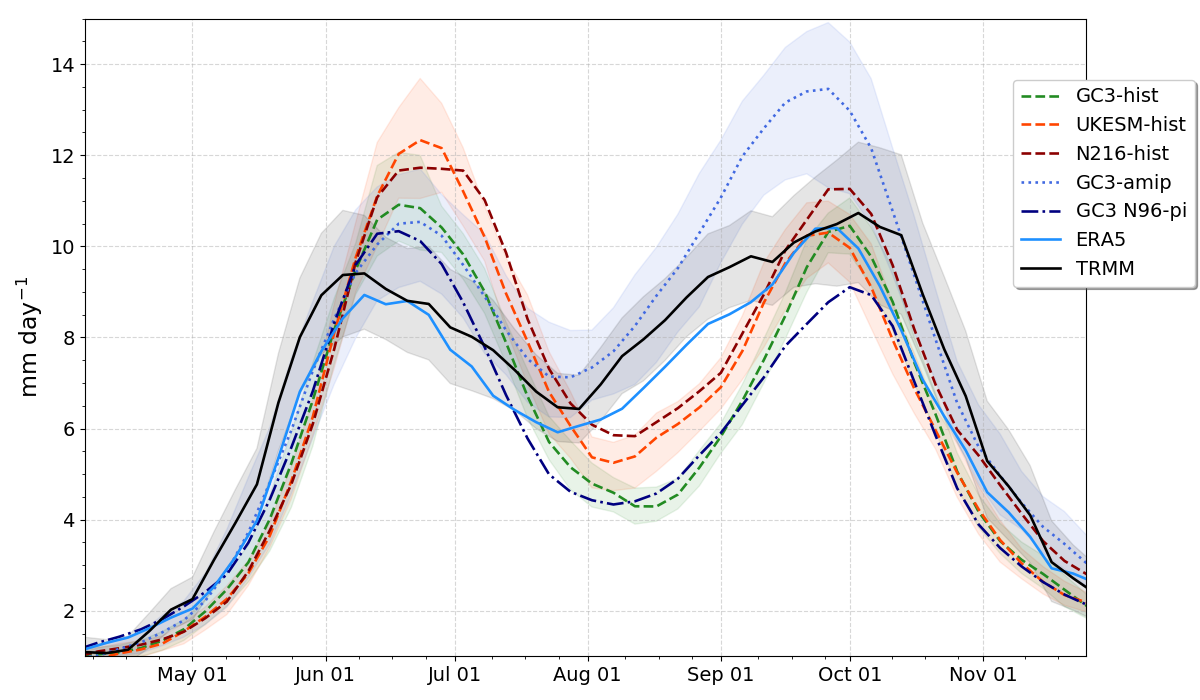
\includegraphics[width=\linewidth]{figures/seasonal_cycle_p3.png}
\caption[Seasonal cycle of precipitation in Mesoamerica]{Pentad-mean precipitation in southern Mexico and northern Central America [95-86$^\circ$W,11-19$^\circ$N]. The shading for the TRMM dataset is a measure of observational uncertainty obtained by bootstrapping the interannual variability whereas the shading for the CMIP6 experiments show the ensemble spread where multiple ensemble members where available. }
\label{fig:msdcaribb}
\end{figure} 
 

This chapter aims, firstly, to improve our understanding of the physical mechanisms associated with the 'real world' MSD of southern Mexico and northern Central America, also referred to as Mesoamerica. A second purpose of this chapter is to diagnose relevant processes that the CMIP6 MOHC accurately simulate in order to capture the seasonal cycle of precipitation. 
For this purpose, the wavelet transform (WT) method introduced in the previous chapter is used to separate the different stages of the rainy season in Mesoamerica in order to capture the dynamic and thermodynamic changes that occur during the seasonal cycle. 

 \begin{figure}[t!]
 \centering
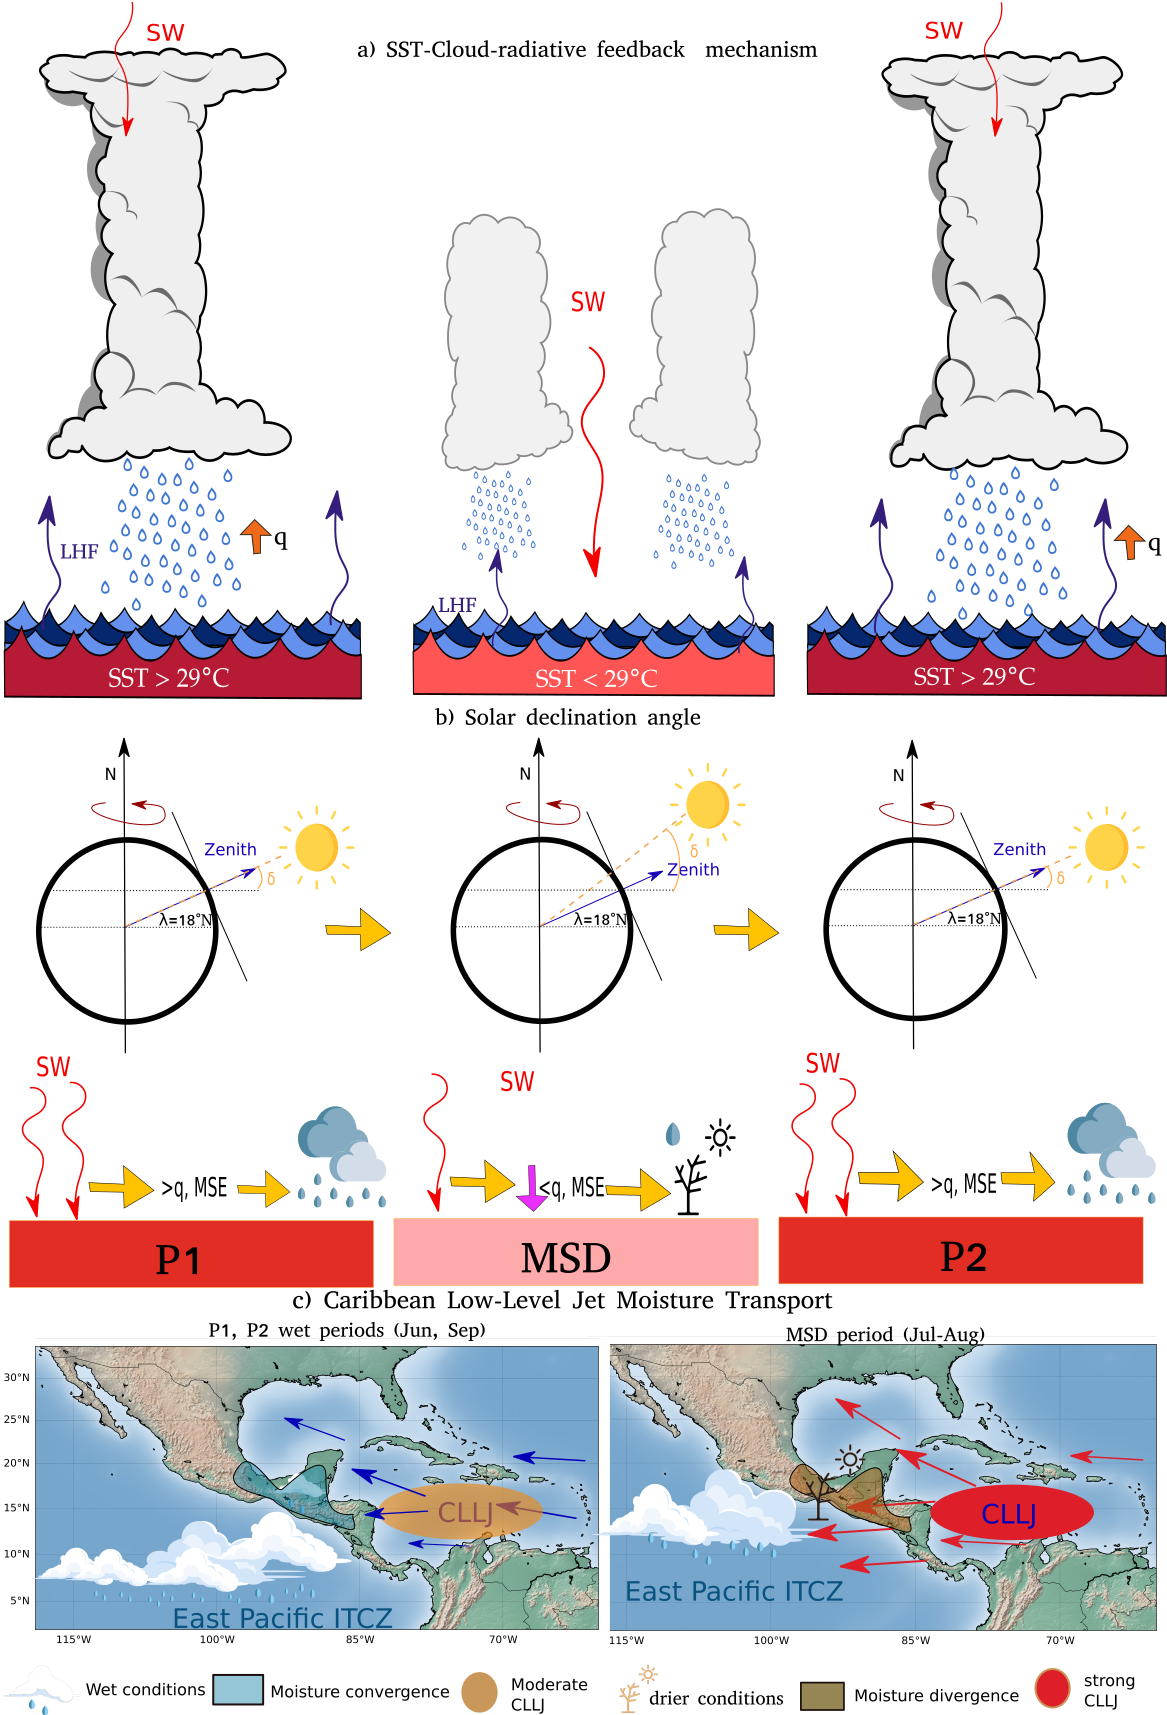
\includegraphics[width=0.84\linewidth]{figures/msd_all_schematics.png}
\caption[Schematics of MSD mechanisms.]{Schematic of the three mechanisms analysed in this chapter, a) the SST cloud-radiative mechanism, (b) the solar declination angle and (c) the moisture divergence mechanism driven by the CLLJ.}
\label{fig:schematic_msd}
\end{figure} 
 

Three leading hypotheses (section \ref{sq:litmsd}) are investigated for the MSD of southern Mexico and Central America:
the SST-cloud-radiative feedback proposed by \cite{magana1999}, the solar declination angle hypothesis \citep{karnauskas2013} and the CLLJ as a modulator for moisture transport and convective activity in Mesoamerica \citep{herrera2015,zermeno2019}.
The main features of the three mechanisms are illustrated in Figure \ref{fig:schematic_msd}. 
Briefly, the cloud-radiative feedback mechanism (Fig. \ref{fig:schematic_msd}a) proposes that the peaks and trough of precipitation in the seasonal cycle are a result of a similar seasonality in the East Pacific SSTs and surface humidity. 
During the first peak of precipitation, cloud radiative effects block shortwave solar radiation from reaching the surface in addition to increased latent heat fluxes from the ocean to the atmosphere cooling the SSTs and leading to a decrease in convective activity and precipitation in the MSD.
During this drier period, incoming shortwave increases again and raises East Pacific SSTs above 29$^\circ$C and surface humidity leading to the second peak of precipitation. %In this framework, the driving mechanism are surface fluxes controlled by the SSTs. %This mechanism relies on the SSTs being related to surface fluxes which are the driving mechanism 

The solar declination angle hypothesis (Fig. \ref{fig:schematic_msd}b) argues that total shortwave radiation absorption at the surface is the key element that controls the surface energy balance and the strongest control of the seasonal cycle of incoming shortwave is the solar declination angle. The total shortwave absoprtion by the surface modifies the surface moist static energy, specifically the surface moisture, which in this framework is the ultimate control of precipitation. In Central America, the solar declination angle crosses twice during the summer, once at the start and once at the end, and evidence by \cite{karnauskas2013} suggests that precipitation follows the solar declination angle and surface moist static energy with a lag of a few weeks.

Finally, the third mechanism investigated in this chapter argues that the seasonal cycle of the CLLJ, possibly influenced by the seasonal variations to the North Atlantic Subtropical High, modifies moisture transport in the region (Fig. \ref{fig:schematic_msd}c). In particular, studies have noted that the increase in the jet strength at the midsummer coincides with a reduction of rainfall over mainland, the MSD. This argument appears more frequently in studies to explain the MSD of the Caribbean \citep{martinez2019}, but suggestions have also been made that the CLLJ variations could control the total moisture transport over the continent \citep{herrera2015}. Especifically, the hypothesis is that during the MSD the strengthening of the CLLJ decreases the convergence of moisture over the continent and the total water content over western Central America, which ultimately explains the slight decrease in precipitation.

These hypotheses are tested in the newest reanalysis of ECMWF (ERA5) and in a subset of CMIP6 experiments with different representations of the MSD seasonal cycle (Figure \ref{fig:msdcaribb}). 
Furthermore, a moist static energy budget framework is implemented, toward the end of the chapter, to determine whether this methodology can provide new insight into the mechanisms that drive variability of precipitation within the rainy season. 
 


 
The remainder of this chapter is presented as follows. Section 2 describes the observational data and the CMIP6 experiments used in this chapter and an overview of how the WT method is implemented to diagnose the timings of MSD. Then, section 3 evaluates the representation of the key features of the regional climate in the CMIP6 experiments and in ERA5.
Then, the roles of the East Pacific SSTs (section 4), cloud-radiative effects and surface shortwave absorption (section 5) and the CLLJ and moisture transport (section 6) are investigated using composite and regression analysis. Finally, a short investigation of the MSD using the moist static energy budget is given in section 7. A summary and discussion is presented in the final section of this chapter. 
  
 % , particularly of the simulated processes that cause the sub-seasonal variations of precipitation  as well as the differences between experiments with varying forcing and different horizontal resolution will also provide relevant information about the simulated current and future response to greenhouse forcing as well as highlight relevant biases in the region for model development. 





%Convective quasi-equilibrium (CQE) and moist static energy (MSE) budgets have been succesfully implemented in monsoon regions to understand mechanisms that drive precipitation changes. The remaining section of this chapter uses MSE and CQE diagnostics to evaluate the role of thermodynamics and ascent within the moist column of the MSD for the seasonal changes to precipitation. 


\section{Data and methods}

\subsection{Observations and reanalysis data}

All the data used in this chapter are described in chapter \ref{ch:3-methods}. In particular, this chapter uses the gridded precipitation datasets of TRMM and CHIRPS. However, the main precipitation dataset will be the reanalysis ERA5. The remaining diagnostics are taken from ERA5 at the 0.75$^\circ$ resolution and for the period 1979-2019. ERA5 precipitation data is used throughout this chapter to compare against the models, and not observed datasets, because of two reasons. Firstly, observational (satellite or surface station) data of all diagnostics are not available on long periods at the daily resolutions required for this study, for example of the wind flow or moisture profiles over the ocean region. Secondly, ERA5 precipitation in the MSD region closely follows TRMM and CHIRPS (Fig. \ref{fig:msdcaribb}), and the previous chapter shows that ERA5 reasonably reproduces the mean timings for the MSD compared to TRMM and CHIRPS. Therefore, ERA5 can be compared to the simulations as another model; one that is more realistic as the reanalysis is partially driven by the observed state of the atmosphere through the assimilations of radiosondes taken in the region as well as satellite data of various quantities \citep{era5hersbach}.

\subsection{CMIP6 data}\label{sq:ch6cmipdata}

This chapter uses the output from realizations of the HadGEM3 GC3.1 run at two resolutions at N96 and N216 and from UKESM1. These experiments are described in section \ref{sq:cmip6exp} and summarised in Table \ref{tab:Sexps}. This chapter follows the terminology and acronyms outlined in section \ref{sq:cmip6exp}. In addition to the pre-industrial, AMIP, and historical experiments used in previous chapters, this chapter uses experiments from the Cloud-Feedback MIP (CFMIP) \citep{webb2017} and ScenarioMIP \citep{o2016} activities of CMIP6 (see Table \ref{tab:Sexps}). These are the GC3-amip lwoff, amip-p4K and amip-m4K from CFMIP, all run at N96 resolution for HadGEM3, and SSP1, SSP2 and SSP5 from the ScenarioMIP for UKESM1, HadGEM3 N96 and N216.

\subsection{Determination of the timings of the MSD}

 \begin{figure}[t!]
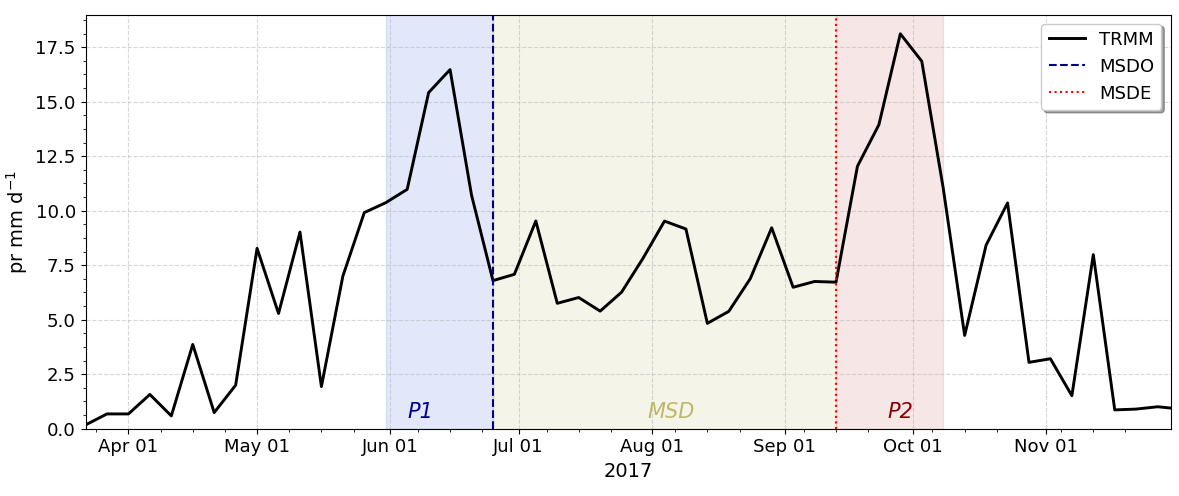
\includegraphics[width=\linewidth]{figures/explain_fig_msd.png}
\caption[Illustration of the use of the wavelet transform method]{Pentad-mean precipitation averaged over the study region [95-86$^\circ$W,11-19$^\circ$N] in the TRMM dataset for the summer of 2017. The timings of the onset (MSDO) and end (MSDE) of the MSD, as well as the first (P1) and second (P2) peak periods and the MSD periods are highlighted. }
\label{fig:explain_msd}
\end{figure}

Chapter 5 describes a wavelet transform (WT) method that can determine the timings of the MSD in observational gridded datasets, reanalysis and climate model precipitation time-series. 
This chapter uses the WT method to determine the onset (MO) and retreat (MR) of the monsoon rainy season, as well as the onset  (MSDO) and end (MSDE) of the MSD. 

To summarise MO and MR are determined by the maximum and minimum sum of WT coefficients computed from a dilation scale vector ranging from 24 to 54 pentads. After MO and MR are determined, a second WT is computed with dilation scales from 10 to 24 pentads and the minimum sum of the WT coefficients corresponds to the onset of the MSD and the maximum to the end of the MSD (MSDE). 
Similarly, the timings of the first (P1) and second (P2) peaks of precipitation are determined from the results of the WT method: P1 is defined as the period between the MSDO and the preceding 4 pentads or 20 days, whereas the second peak is defined as the period between the date of MSDE and the subsequent 4 pentads. An example of this separation of the MSD timings for each year is given in Figure \ref{fig:explain_msd}, for precipitation observed from TRMM in 2017 over the study region.

The area of study of this chapter is in southern Mexico and northwestern Central America (depicted in Figure \ref{fig:eof2}) a region with strong and robust MSD signals (see Chapter \ref{ch:5-wvt}). The WT method was applied to the TRMM, CHIRPS and ERA5 datasets and in the model precipitation time-series area-averaged over the study region. 

  \begin{figure}[b!]
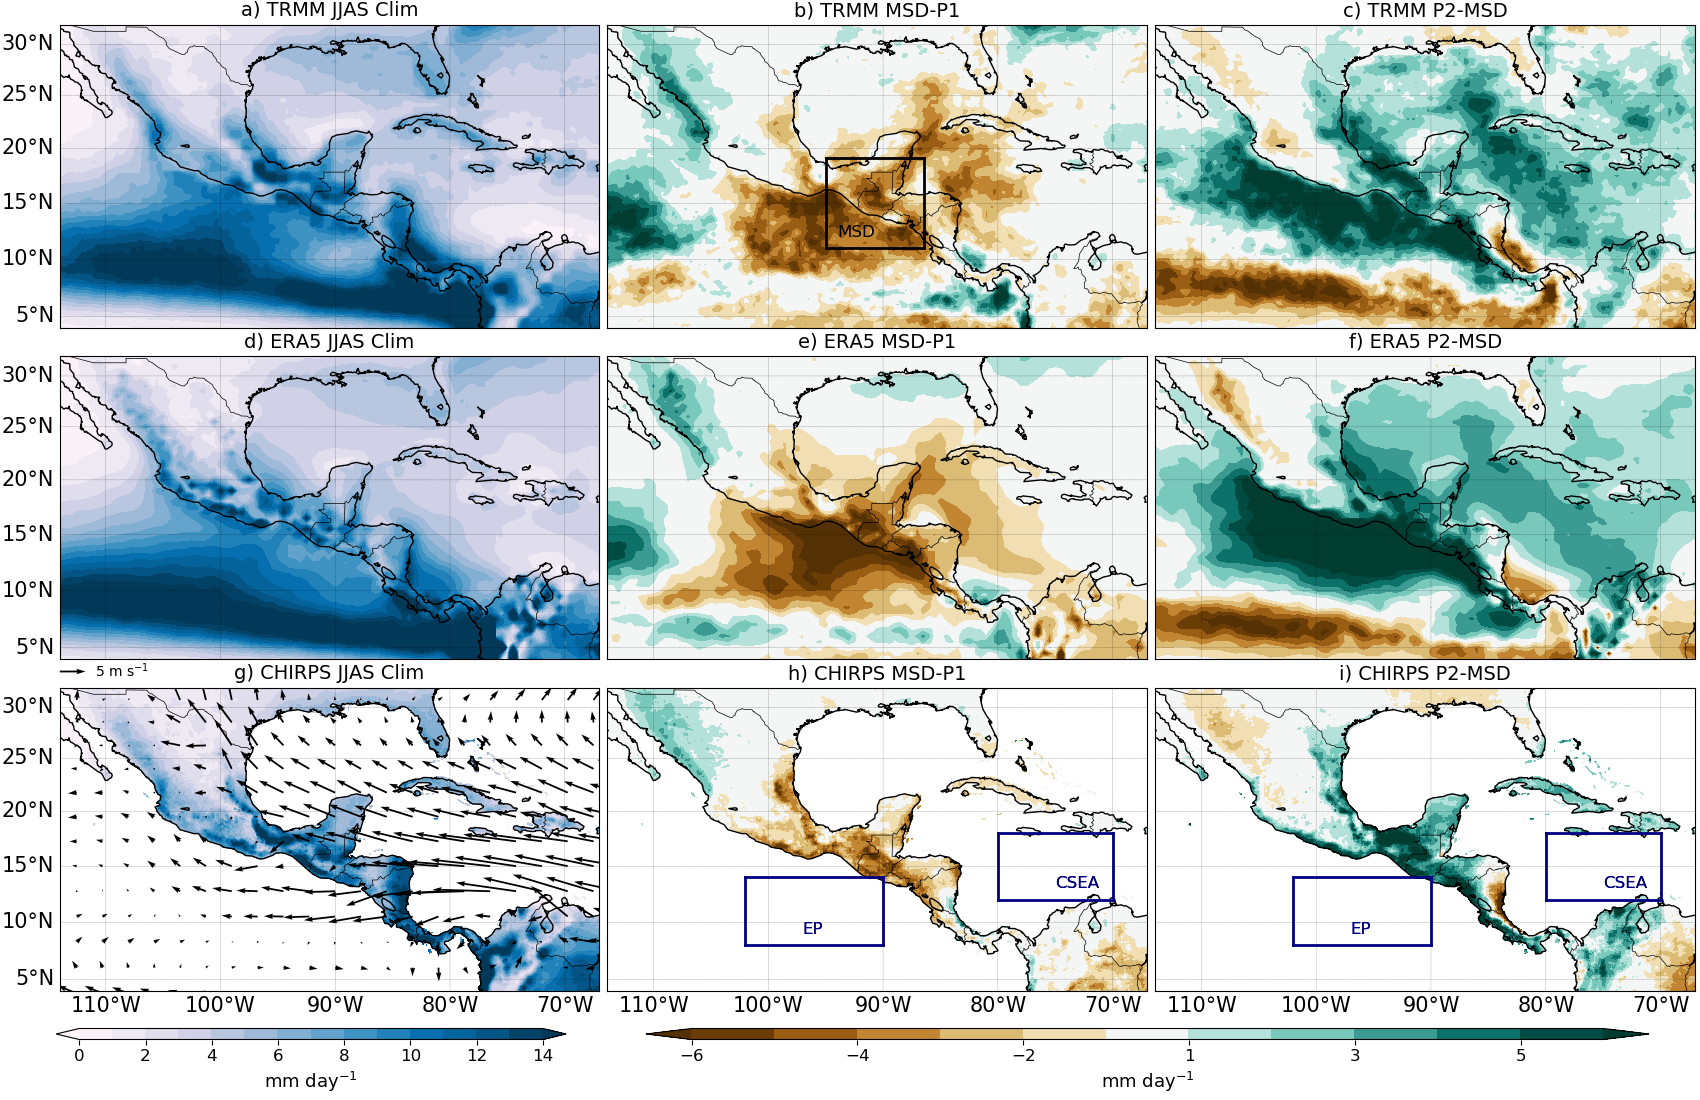
\includegraphics[width=\linewidth]{figures/fig2obs_prdiff_2.png}
\caption[Observed composites of climatological and seasonal variations of precipitation.]{ (a, d, g) Climatological JJAS rainfall and the difference between  (b, e, h)  the midsummer drought and the first peak (MSD-P1) periods and (c, f, i)  between the second peak and the midsummer drought (P2-MSD) periods for (a-c) TRMM, (d-f) ERA5 and (g-i) CHIRPS. The climatological low-level winds (at 850 hPa) for JJAS in ERA5 are shown in c). The boxes in panels b, h and i show the definitions of the MSD, EP and CSEA regions that are used throughout this chapter.  }
\label{fig:eof2}
\end{figure} 

\section{Climatological features}

\label{sq:msdclim}



The seasonal cycle of precipitation in the MSD region (Figure \ref{fig:msdcaribb}) is reasonably well simulated by the CMIP6 experiments and by ERA5, as shown in previous chapters.
The two-peak structure of the MSD is observed in TRMM and ERA5 as two precipitation maxima, the first peak found during early to mid-June and the second peak at the end of September, separated by a drier period that spans from late June to late August. The precipitation in ERA5 not only closely follows the precipitation variations at the pentad scale but also generally agrees with the mean precipitation rate during the first peak, the MSD and second peak periods.

The MSD period in the CMIP6 experiments is observed one or two pentads after TRMM and ERA5 (see the mean values in the previous chapter) and shows a stronger variation of precipitation between the first peak and the Midsummer. A noteworthy difference is that the timing of the MSD is better represented in GC3-amip, particularly the MSDE date, suggesting a role for the SST variability or biases being relevant.
In general, the pre-industrial control experiments show a higher magnitude of precipitation during the first peak and the MSD period whereas GC3-amip experiments are characterized by a wetter second peak. 

\begin{figure}[t!]
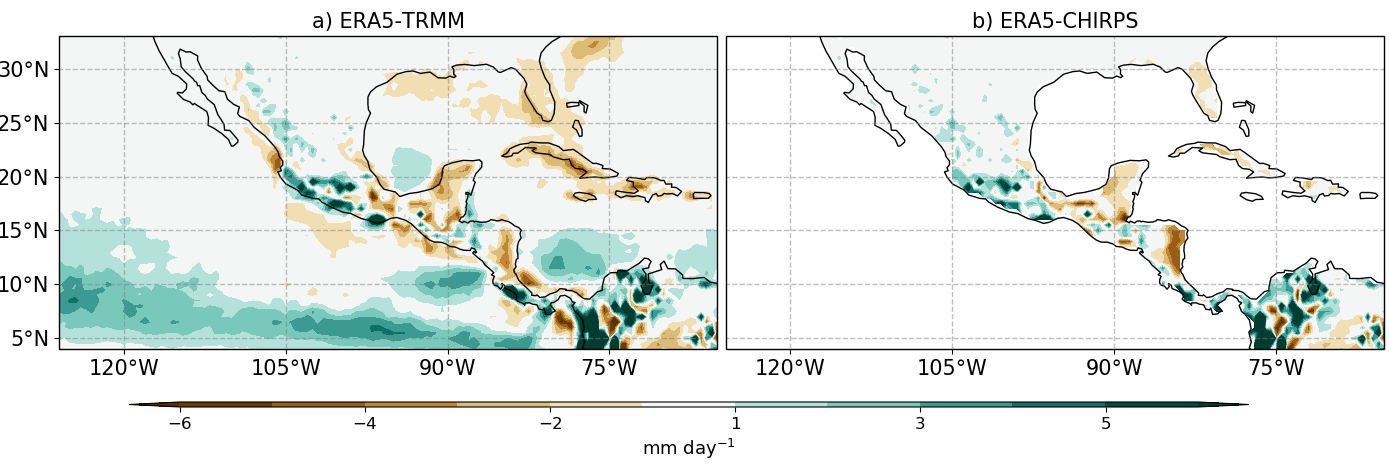
\includegraphics[width=\linewidth]{figures/fig_Era5}
\caption[ERA5 precipitation biases]{ (a, b) JJAS precipitation biases in ERA5 when compared to (a) TRMM and (b) CHIRPS. }
\label{fig:era5_bias_pr}
\end{figure}
 
 The climatological distribution of precipitation and the temporal differences within the MSD timings in ERA5 agrees well with TRMM and CHIRPS (Figure \ref{fig:eof2}). ERA5 reasonably captures the climatology of precipitation over land in Mesoamerica but also captures the strength and position of the East Pacific ITCZ, as shown by the precipitation maximum in the easternmost Pacific (panels a, d).  Specifically, the biases of JJAS-mean precipitation in ERA5 are shown in Figure \ref{fig:era5_bias_pr}. While positive biases are found over the East Pacific Ocean, negative (weaker) biases are found over land in southern Mexico and Central America.
 
  The patterns of the MSD-P1 and P2-MSD differences in ERA5 (Fig. \ref{fig:eof2}) also agree well with TRMM. These two panels show that precipitation differences associated with the MSD measured by the area-averaged precipitation within the box in Figure \ref{fig:eof2}b extends outside of the study region all over the Intra-Americas Seas comprising the easternmost Pacific Ocean, the entrance to the Gulf of Mexico and western Caribbean Sea, particularly in the P2-MSD panel. Notably, the strongest differences for both panels are found on the western coast of Mesoamerica. 
 
 
\begin{figure}[t!]
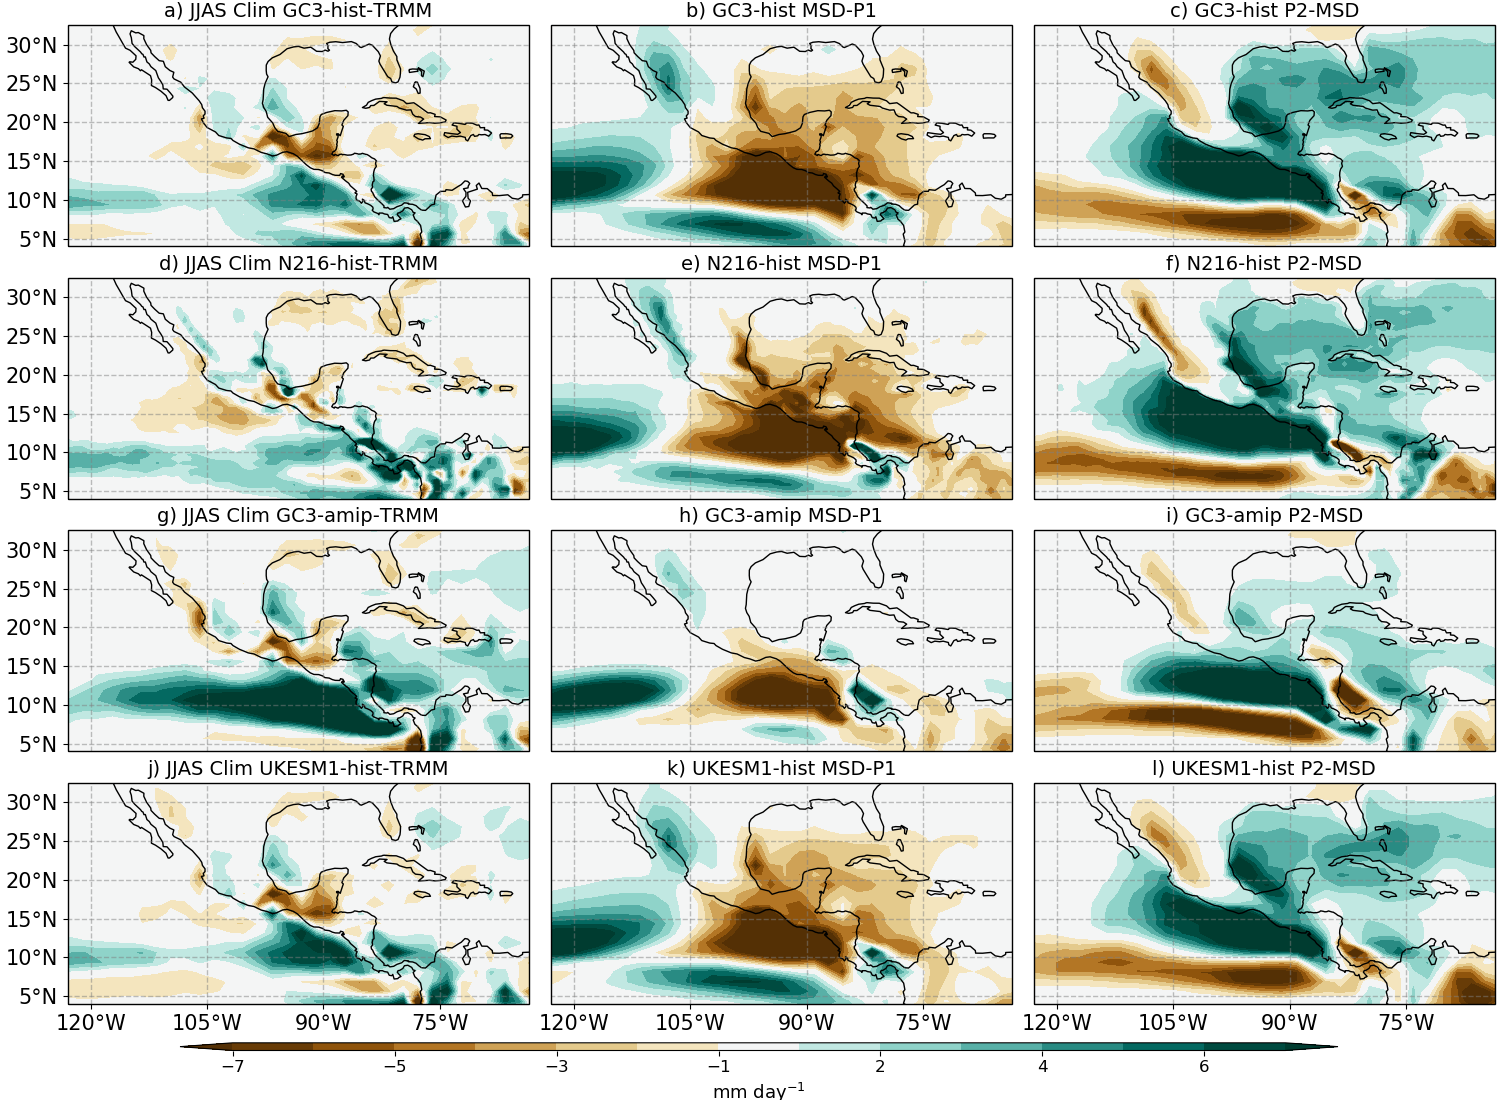
\includegraphics[width=\linewidth]{figures/fig2obs_prmodels3}
\caption[Composite mean precipitation biases and seasonal variations]{ (a, d, g, j) JJAS model bias compared to TRMM and the difference between  (b, e, h, k)  the midsummer drought and the first peak periods and (c, f, i, l)  between the second peak and the midsummer drought periods for four different simulations.}
\label{fig:model_pr}
\end{figure} 
 
 In turn, the simulations (Figure \ref{fig:model_pr}) have important biases in the magnitude of the  precipitation in the East Pacific ITCZ with a positive bias of 3-6 mm day$^{-1}$ depending on the simulation as well as a dry bias over southern Mexico and Central America, as shown in chapter \ref{ch:4-ams}. These biases are much larger than the biases between ERA5 and TRMM and CHIRPS.
The simulations capture the spatial patterns associated with the MSD stages, which also show the strongest differences are found on the west coast of the Mexican state of Chiapas, Guatemala and El Salvador. The negative differences in the MSD-P1 and positive differences in the P2-MSD extend to the Caribbean Sea, northeastern Mexico and the Gulf of Mexico. 
In agreement, with ERA5 and TRMM, the simulations show that the precipitation differences in the MSD region are always opposite to that of the North American monsoon region, e.g., in Figures \ref{fig:eof2} and \ref{fig:model_pr} the North American monsoon is wetter when the MSD period begins and Mesoamerica is drier.
  
 
 
\label{sq:msdclim}
 \begin{figure}[t!]
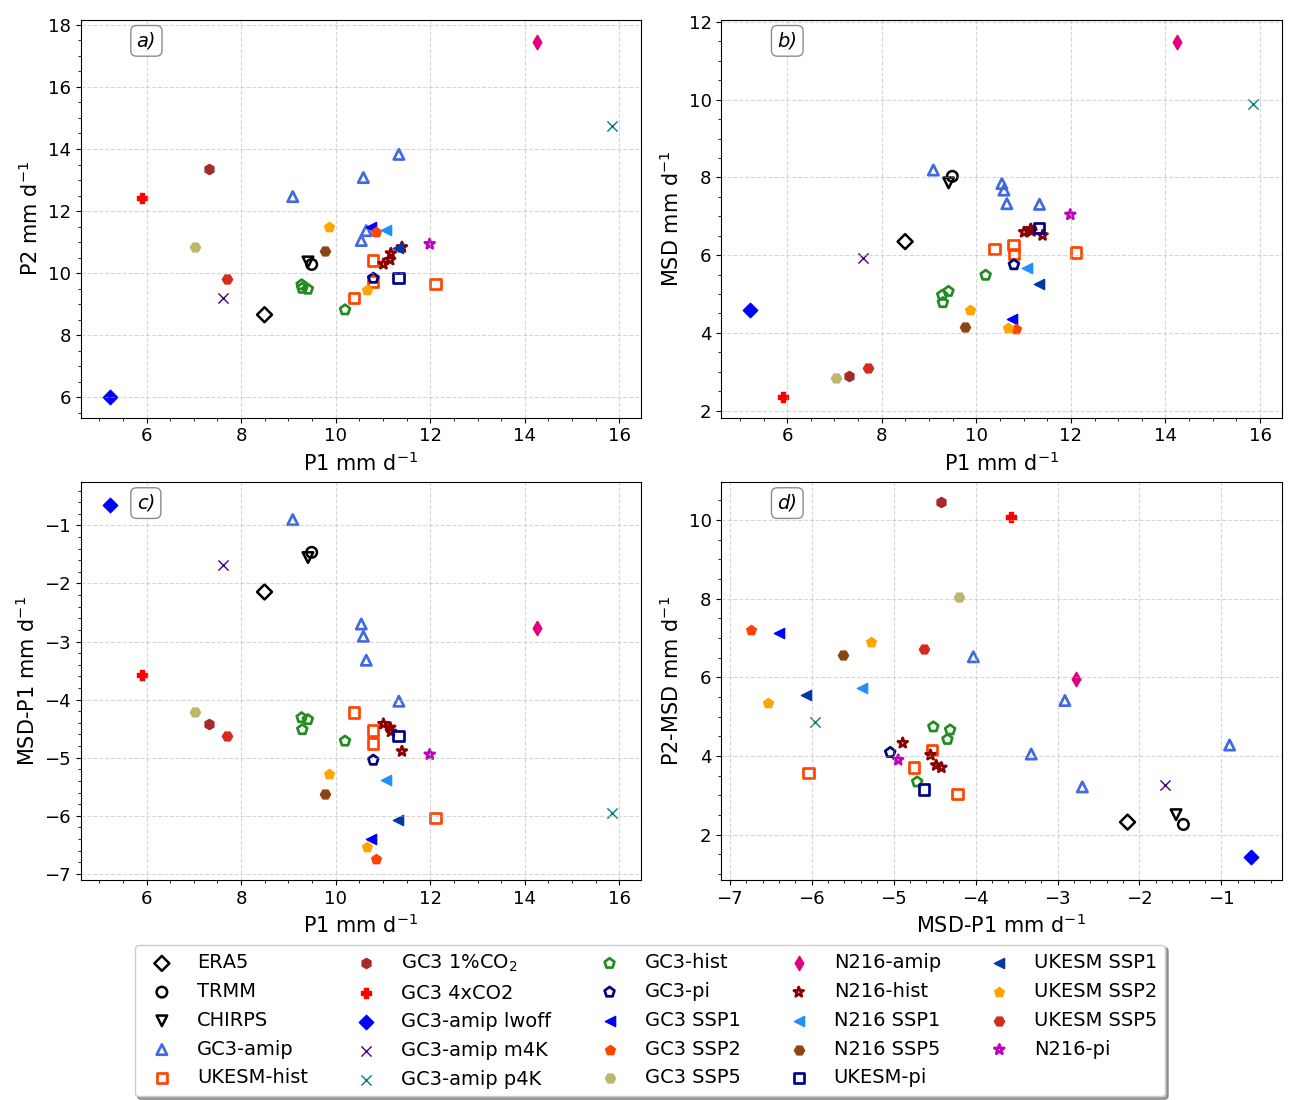
\includegraphics[width=\linewidth]{figures/dumscatter_2.png}
\caption[Scatter plot of mean precipitation in different parts of seasonal cycle]{(a, b) Scatter plots of the mean values of precipitation [mm day$^{-1}$] for TRMM, ERA5, CHIRPS and the CMIP6 experiments (see \ref{sq:ch6cmipdata}) during the first peak (P1), the MSD and the second peak (P2) periods and (c, d) the precipitation differences between the three periods. The region used for this averages if illustrated in Figure \ref{fig:eof2}.  
  }
\label{fig:scatter_msd}
\end{figure} 

The mean rainfall observed in the three periods (P1, P2 and the MSD) in the simulations varied notably between experiments done with different model configurations and with external forcing (Figure \ref{fig:scatter_msd}). 
 The scatter of the first and second peak and the MSD mean rainfall rates  shows, first, that the mean rainfall in each stage is not linearly related to another, i.e., a larger magnitude of the first peak of precipitation does not necessarily imply a wetter or drier MSD period. The atmosphere-only runs, GC3-amip, is a good example of this behaviour as the mean rainfall during P1 is roughly the same as in the rest of the simulations but the mean rainfall during the MSD is slightly larger than in the rest of the simulations and the P2 precipitation is largest in GC3-amip. 
 
 
Second, the magnitude of the first decrease in rainfall (MSD-P1) and the late-summer increase (P2-MSD) also show a significant spread amongst experiments, which also suggest that there is no clear association between the magnitude of the MSD and the magnitudes of the two peaks of precipitation in these simulations. The scatter of ERA5 in all panels is notably close to that of TRMM and CHIRPS, which is further evidence that the timings and strength of the MSD is well represented by this reanalysis. In contrast, the high resolution atmosphere-only run (N216-amip) shows the highest bias in precipitation throughout the three stages of the wet season. This result is noteworthy because this configuration uses the medium-resolution atmosphere and ocean, i.e., a higher resolution than GC3 amip and is forced by observed SSTs, the simulation cannot capture the observed precipitation rates and is strikingly the worst simulation overall. %, even worse than idealized experiments such as the abrupt 4$\times$CO$_2$ experiment. 

 %In observation and reanalysis, the interannual variability shows a similar behaviour, i.e., the magnitude of precipitation at each stage is not related to the next stage (not shown). 

 \begin{figure}[t!]
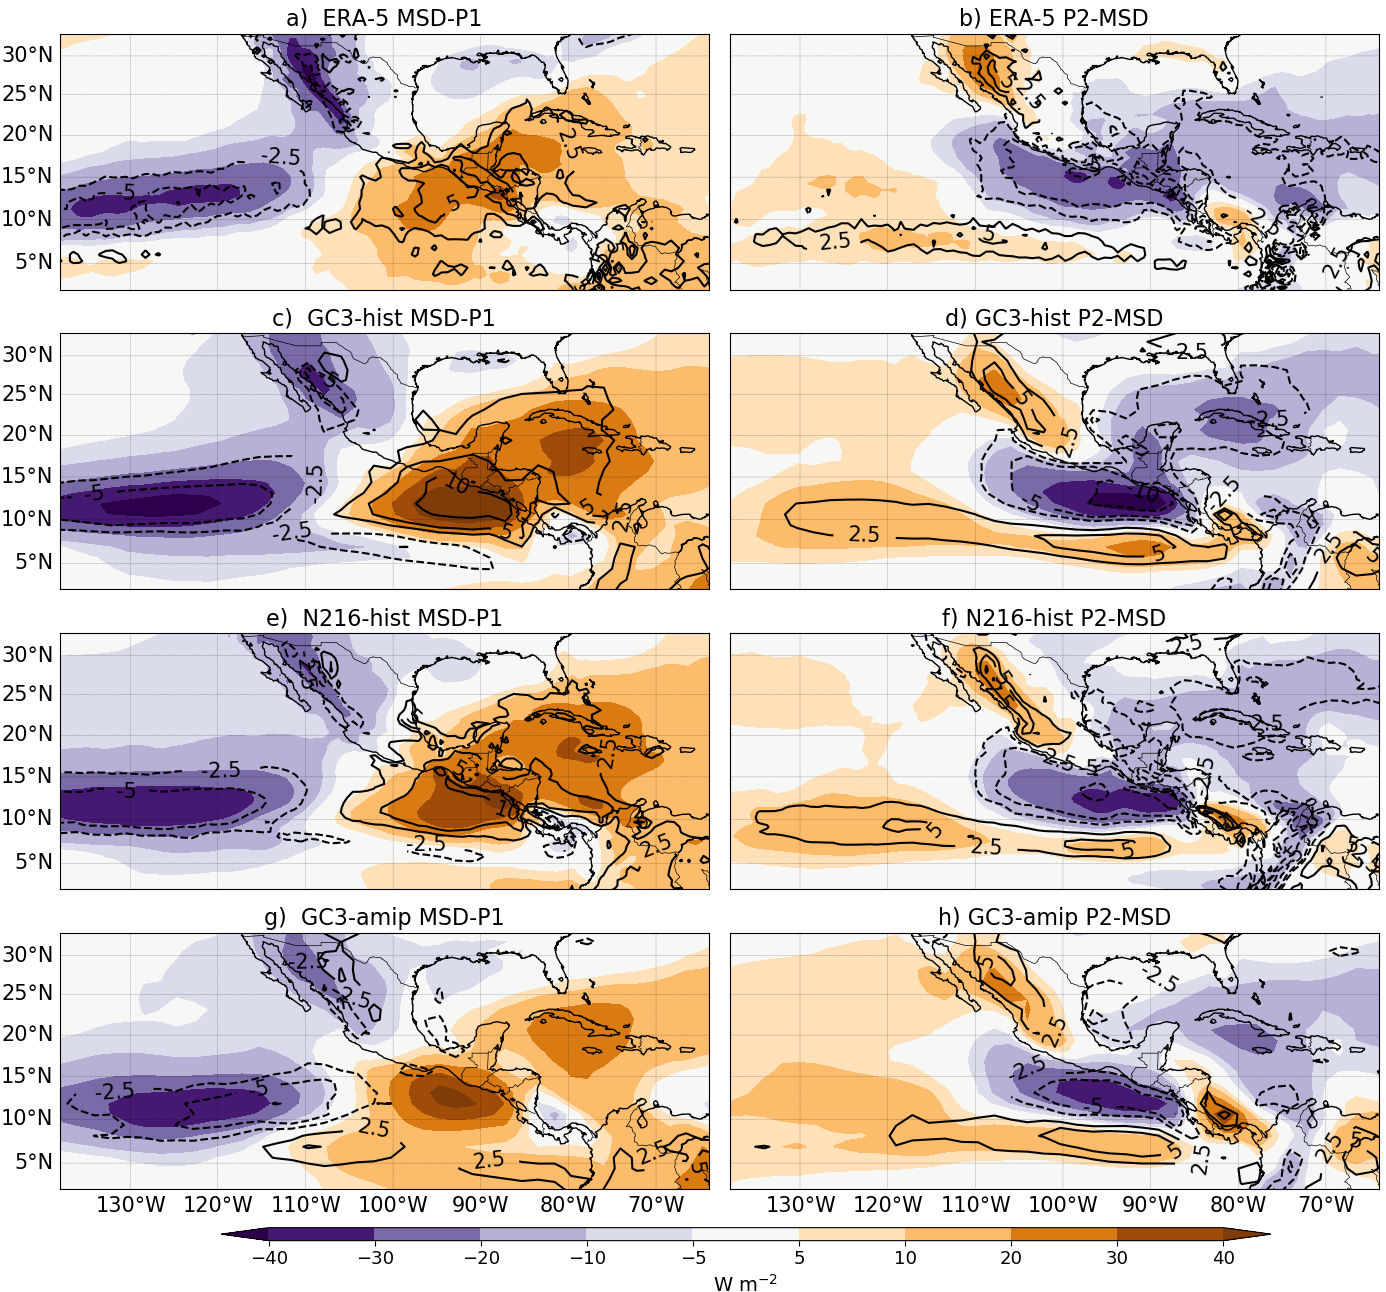
\includegraphics[width=\linewidth]{figures/fig4_olrv_3.png}
\caption[OLR and vertical velocity composites]{Outgoing long-wave radiation (OLR) [W m$^{-2}$] (shaded) and $\omega$ 500-hPa [$10^{-2}$ Pa s$^{-1}$] (line contours) differences between the MSD and first peak and the second peak and MSD.}
\label{fig:olranom}
\end{figure}

 The outgoing long-wave radiation (OLR) and vertical velocity ($\omega$ at 500 hPa) differences associated with the MSD were computed using the WT method for each dataset (Figure \ref{fig:olranom}). These composite results also show that the MSD is not a local-scale feature but convective activity varies coherently in neighboring regions. From the first peak period to the MSD, OLR and $\omega$, increase notably in the easternmost Pacific, southern Mexico and northern Central America and extend into the Caribbean islands and Sea, and in the case of OLR into the North Atlantic; because $\omega$ is defined as $\omega=DP/Dt$  these positive anomalies are indicative of weaker convection. 
 
 In contrast, two regions show opposite responses to the MSD. A region several degrees west of land (125$^\circ$W) and another region north of the study region, i.e., the North American monsoon region, show signs of negative OLR and $\omega$ anomalies, in the MSD-P1 panels. These negative anomalies are indicative that, simultaneously to the onset of the MSD,  convection is observed stronger and deeper in the North American Monsoon region and in the Pacific region west of the continent; the stronger convection found at around 125$^\circ$W was also described by \cite{herrera2015}. 
 
 \begin{figure}[t!]
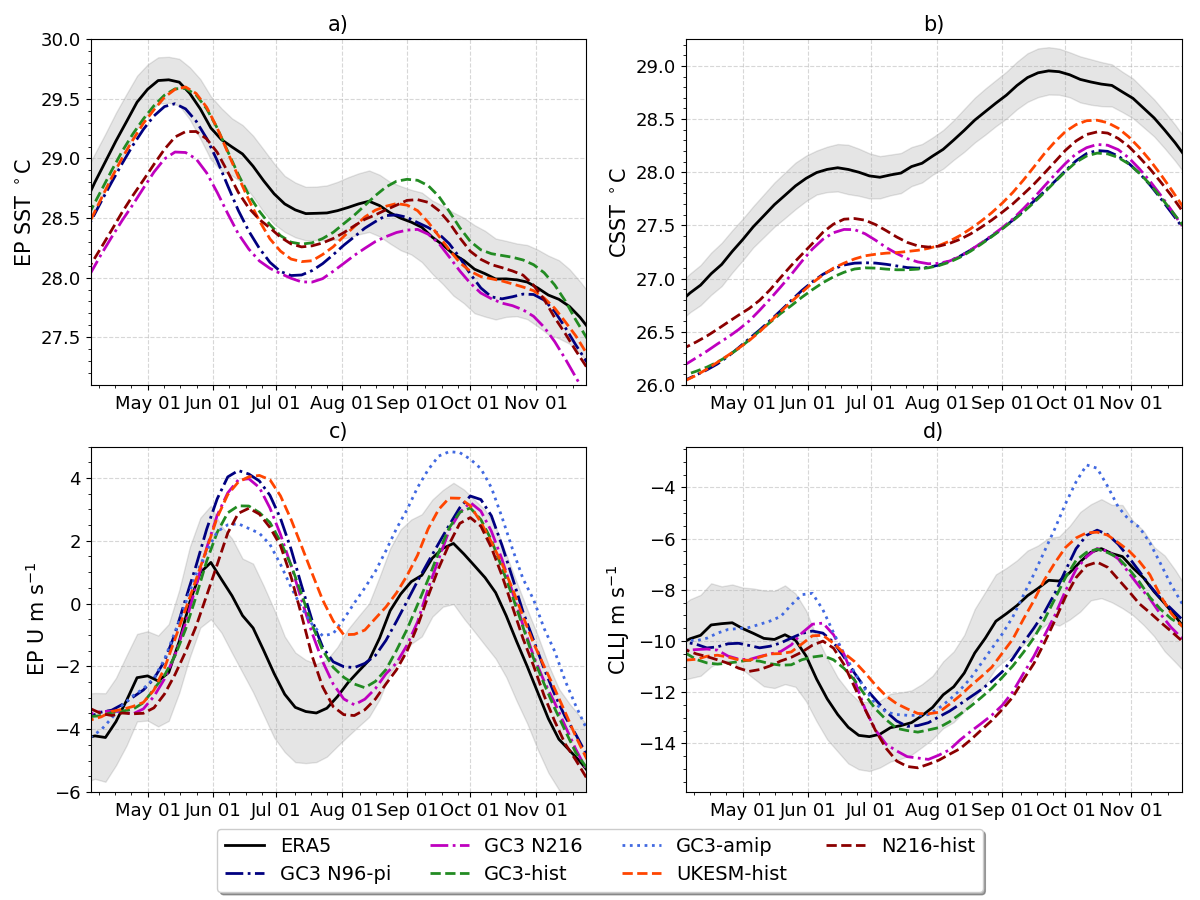
\includegraphics[width=\linewidth]{figures/index_seasonal}
\caption[Seasonal cycle of East Pacific and Caribbean SSTs and zonal winds.]{Pentad-mean seasonal march of the (a, b) SSTs [$^\circ$C] and (c, d) the low-level (925-hPa) zonal wind flow [m s$^{-1}$] in (a, c) the easternmost equatorial Pacific and (b, d) the Caribbean Sea. The transparent shading is as in Figure \ref{fig:msdcaribb}. The regions used for EP and CSEA averages are illustrated in Figure \ref{fig:eof2}h.}
\label{fig:csst}
\end{figure}
 
 
 The OLR and $\omega$ variations associated with the end of the MSD show a relatively opposite picture to the MSD-P1 differences (Fig. \ref{fig:olranom}). OLR and $\omega$ decrease all across the central and south western coast of Mexico and northern Central America extending into the Caribbean Sea whereas positive differences are found in the North American Monsoon region and in the Pacific Ocean at around 125$^\circ$W.  These composites agree with the results of \cite{herrera2015} that argues that ascending and descending anomalies in the MSD are closely related to ascent and descent elsewhere.

The literature suggests that a number of climatological features of the region play key roles for the MSD (Section \ref{sq:litmsd}). These climate features include the seasonal cycle of the East Pacific (EP) SSTs, the Caribbean Sea SSTs, the Eastern Pacific zonal wind flow and the CLLJ \citep{magana1999,amador2008,herrera2015,straffon2019,garcia2020sub}. 
The seasonal cycle of these features in ERA5 and the simulations (Figure \ref{fig:csst}) shows that the models are able to replicate the seasonal variations of the SSTs and the zonal wind flow of the region. However, some key biases are observed in the simulations.

The seasonal cycle of EP SSTs (Figure \ref{fig:csst}a) show the maximum peak SST in late May, prior to the first peak of precipitation in Mesoamerica. In contrast, the Caribbean SSTs peak in early fall, about five months later, during late September. After the peak SST period in the EP, SSTs decrease to a local minimum found in July both for ERA5 and the simulations. The models show an overall cold bias in the SSTs in both regions, but this bias is most pronounced in the Caribbean Sea where throughout the wet season the SSTs in the models are colder than in ERA5. 

 The low-level wind flow in the EP shows a bimodal seasonal cycle in both ERA5 and the simulations (Figure \ref{fig:csst}c).
The easterly flow in the EP during the spring becomes weaker turning westerly at the end of May and reaching a local maximum in early June in ERA5 and mid-June in the simulations. This local maximum then decreases during June and early July as the zonal wind becomes easterly again. The easterly flow peaks in mid July in ERA5 and about three weeks later in the simulations. The strength of this easterly flow magnitude during the midsummer varies greatly amongst the simulations. 
After the peak easterly flow in  the midsummer, or zonal wind local minimum, the zonal wind becomes westerly again peaking at the end of September-early August in both ERA5 and simulations. 
This seasonality of the zonal wind in the EP is notably similar to the seasonal cycle of precipitation in the region, and the difference in the phase of ERA5 and the models is also the same between the zonal wind and precipitation.

The CLLJ seasonal cycle (Figure \ref{fig:csst}d) is reasonably replicated by the simulations, compared to ERA5, although the peak strength of the CLLJ, which is found during the last week of June in ERA5, is delayed in the simulations by about three weeks, as the simulated CLLJ peaks in mid-July in all the simulations.
The simulations follow closely the late summer and fall seasonal cycle and magnitude of the CLLJ, except for a notable bias in GC3-amip in Oct-Nov characterised by a weaker than observed zonal wind.

\section{The role of East Pacific SSTs}

 The East Pacific (EP) SSTs are a key element of the radiative-convective feedback mechanism of \cite{magana1999}, which argues that the EP SSTs, cloud radiative effects and surface fluxes are part of a feedback mechanism that explains the two peak structure of the seasonal cycle of precipitation in Mesoamerica. A key prediction of this mechanism is that East Pacific SSTs and surface fluxes exhibit a bimodal  seasonal cycle in which EP SSTs and surface fluxes decrease during the first peak period and increase during the Midsummer drought period. In other words, this hypothesis predicts that the summer march of the EP SSTs should also exhibit a bimodal signal, similar to that observed for precipitation but out-of-phase, with the SSTs leading the precipitation. This section aims to evaluate these predictions for ERA5 and for the CMIP6 experiments. 

 
\begin{figure}[b!]
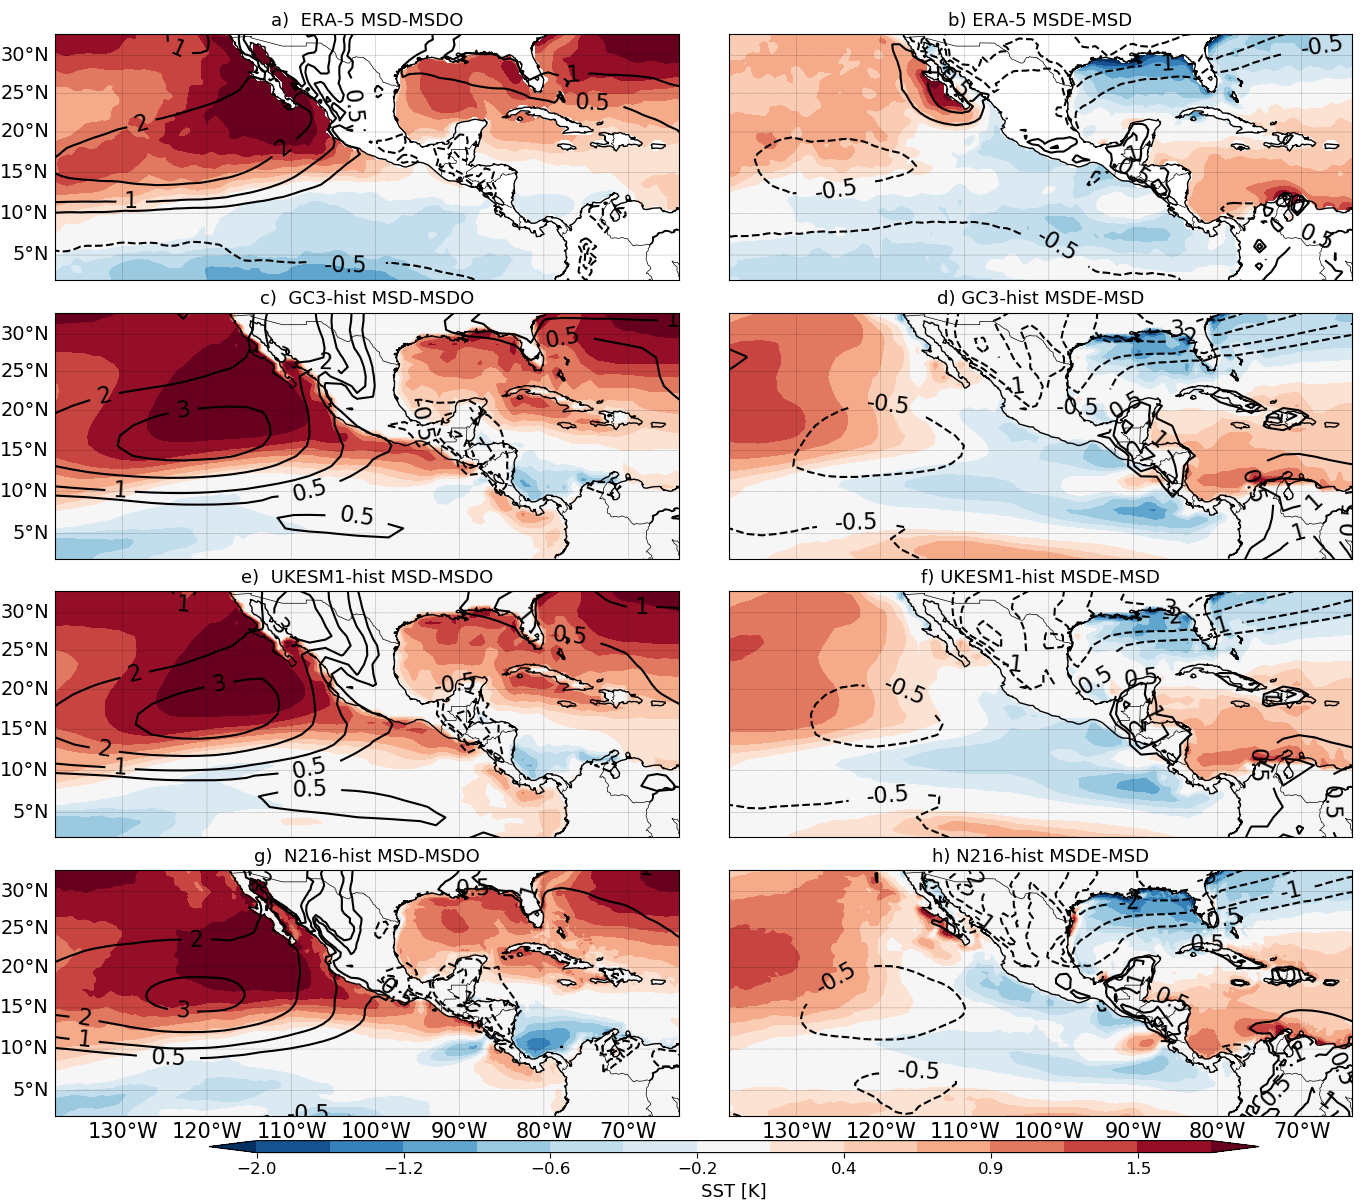
\includegraphics[width=\linewidth]{figures/fig4_sstv_3.png}
\caption[Composite SST anomalies]{As in Figure \ref{fig:olranom} but the anomalies are shown for SSTs [K] (contours) and surface humidity [g kg$^{-1}$] (line-contours).  }
\label{fig:msdsstanom}
\end{figure}

According to the radiative convective feedback mechanism, the EP SSTs should cool down during or slightly prior to the onset of the MSD and then increase during the local minimum of rainfall, i.e., during the MSD period which would lead enhanced precipitation and cause the second peak of precipitation in late summer. However, in ERA5 the EP SSTs only very slightly increase during the MSD (Jul-Aug) and instead of increasing in late summer rather cool again in late August and September. In fact, the EP SSTs in ERA5 decrease after mid-August, in synchrony with the second peak in deep convection and precipitation (Figs. \ref{fig:msdcaribb} and \ref{fig:csst}a).

 In the models, however, there is indeed a second peak in EP SSTs in late summer found in early September and therefore nearly synchronous to the second peak of precipitation. While EP SSTs clearly lead precipitation in May-June, the SST-precipitation relationship in mid and late summer is less obvious. In the models, the second peak of SSTs is nearly synchronous to the second peak in precipitation, which seems to contrast with the predictions of the radiative-convective feedback mechanism.
 
In order to better understand the relationship between EP SSTs and precipitation over the MSD region, the WT method is used to composite SSTs and surface humidity in the P1, MSD and P2 periods. 
The spatial distribution of SST and surface humidity changes associated with the MSD  (Figure \ref{fig:msdsstanom}) suggest that the EP SSTs south of 10$^\circ$N cool slightly between the first peak (P1) and the MSD periods, meanwhile the Gulf of California and the northern eastern Pacific significantly warms. At the end of the MSD (P2-MSD), the EP SSTs decrease in both ERA5 and the simulations. 
The P2-MSD panels also show that the Caribbean SSTs increase, associated with the peak Caribbean SSTs  at the end of the summer (Fig. \ref{fig:csst}b).

The historical simulations generally agree with the composite differences of ERA5, with no appreciable warming in the EP region in the MSD-P1 panels, and cooling in the EP and the Gulf of Mexico and warming in the Caribbean Sea in the P2-MSD panels.
These results suggest that while the seasonal cycle of EP SSTs show a bimodal signal, when each year of each simulation is examined using the WT method, which has proven to skilfully diagnose precipitation variations associated with the MSD, the EP SSTs do not synchronously warm during or after the MSD, as argued by the radiative-convective feedback.


\begin{figure}[t!]
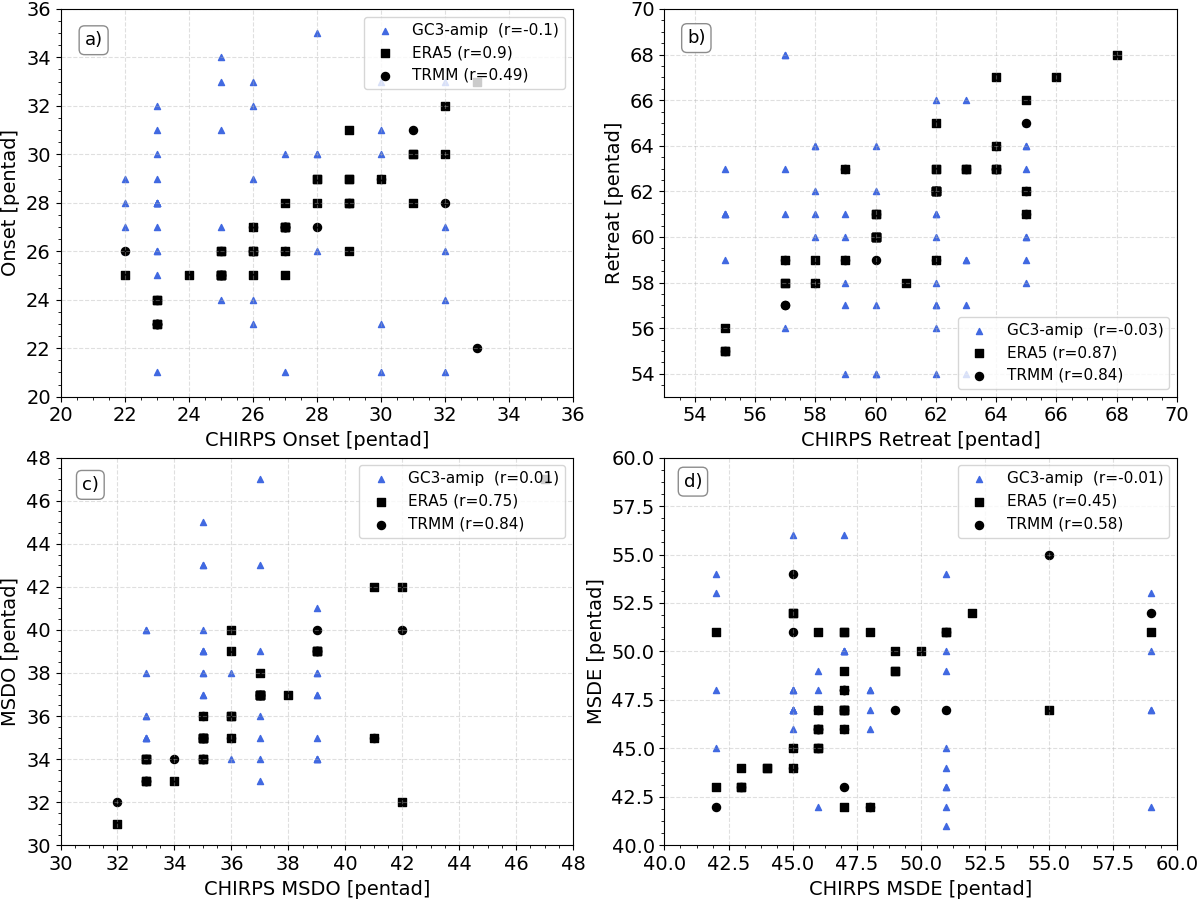
\includegraphics[width=\linewidth]{figures/master_sst_scatter.png}
\caption[Scatter plot of SST vs precipitation]{Scatterplots of the pentads diagnosed by the WT method as the dates of (a) monsoon onset (MO), (b) monsoon retreat (MR), (c) MSDO and (d) MSDE where the results of the CHIRPS dataset, on the x-axis, are compared with ERA5, TRMM and the GC3-amip simulation, on the y-axis. The legend shows the Pearson $r$ coefficient for each comparison. }
\label{fig:amipsstscatter}
\end{figure}


An argument of the feedback mechanism is that the SST variability would force changes to the surface humidity and ultimately precipitation. The surface humidity in the EP and MSD regions, however, is largely unchanged (less than 0.5 g kg$^{-1}$) during the various stages of the MSD (Figure \ref{fig:msdsstanom}), even though precipitation varies notably during these periods. Instead, the greatest variations in surface humidity are observed west of Baja California from the P1 to the MSD, and this region of increased surface humidity extends into the North American Monsoon region. Similarly, at the end of the MSD, the most notable variations in surface humidity is the drying of the North American monsoon region.
 The surface humidity variations in the simulations also agree well with those of ERA5 and are very similar amongst the realizations.



\begin{figure}[t!]
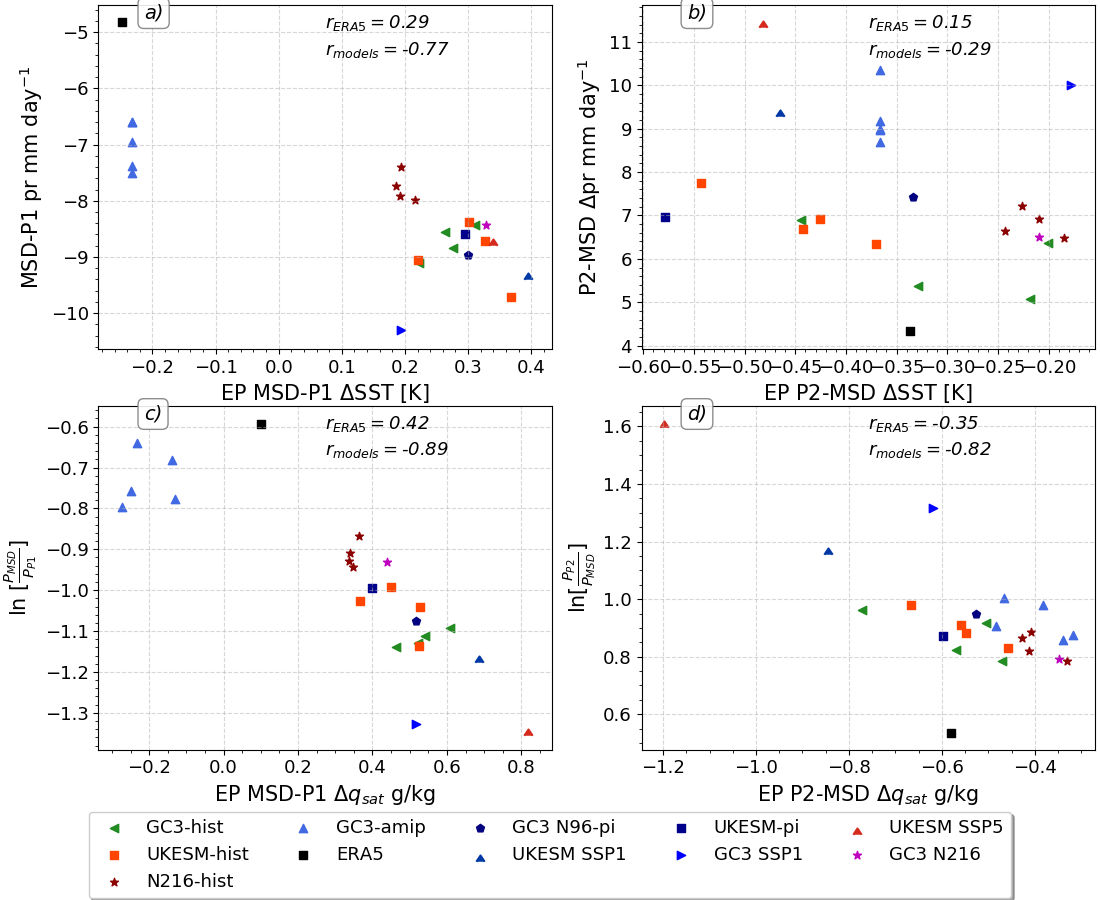
\includegraphics[width=\linewidth]{figures/sst_scatter_f.png}
\caption[Scatter plot of SST changes]{Scatterplots of the mean changes in the East Pacific (a, b) sea-surface temperatures (SSTs) and (c, d) surface saturation specific humidity q$_{sat}$ in the x-axis with respect to precipitation variations in the MSD region on the y-axis for the (a, c) MSD-P1 and (b, d) P2-MSD periods.  The correlation coefficient of the interannual spread in ERA5 and the multi-experiment correlation coefficient are shown in each panel.   }
\label{fig:var_sst_lhf_scatter}
\end{figure}


If the EP SSTs play a dominant role in the timings and strength of the MSD, as implied previously \citep{magana1999,magana2005,herrera2015}, then the simulations with imposed SSTs taken from observations, e.g., the GC3-amip experiment, may be further explored to evaluate the links  between the timings or strength of the MSD in GC3-amip and ERA5. A scatter plot of the dates (pentads) of the MO, MR, MSDO and MSDE (Figure \ref{fig:amipsstscatter}) for matching years between the CHIRPS dataset and TRMM, ERA5 and the five ensemble members of GC3-amip shows that the timings of the MSD in GC3-amip are unrelated to CHIRPS and ERA5. In fact ERA5, in spite of precipitation being largely a model-derived quantity in the reanalysis, produces MSD timings that agree fairly well with the CHIRPS and TRMM datasets. 
This evidence would suggest that the SSTs forcing the model in GC3-amip are not the dominant factor controlling the timings of the MSD in these atmosphere-only runs.

Alternatively, the interannual variability in ERA5 and the differences amongst the MOHC CMIP6 experiments may be further explored to understand whether the changes to the SSTs are related to changes in the precipitation. For this purpose, composite differences between the P1, MSD and P2 periods were computed for each variable for each year in each dataset and then averaged to provide a mean value that relates changes in precipitation to different diagnostics in different stages of the rainy season.   For example, the mean difference in SSTs (Figure \ref{fig:var_sst_lhf_scatter}a) between the P1 and the MSD periods, show a cooling difference for ERA5 associated with a smaller precipitation reduction. In contrast, the coupled model simulations show a positive SST difference (warming) associated with a greater precipitation reduction during MSD compared to the P1 period.


\begin{figure}[t!]
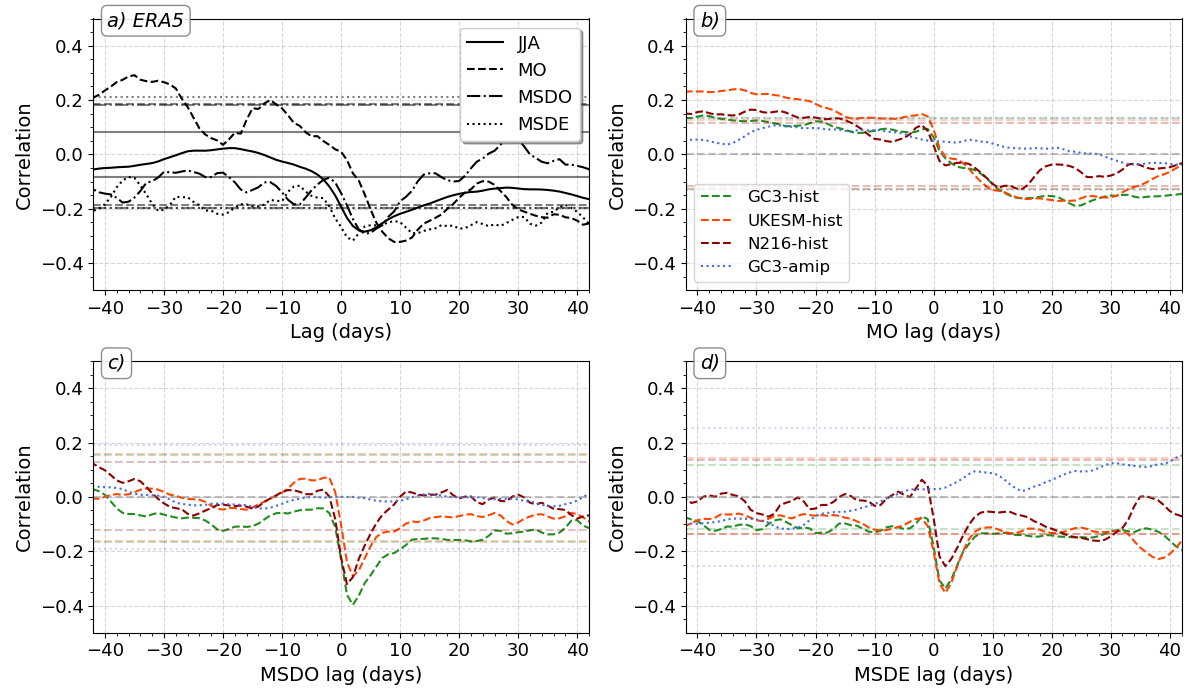
\includegraphics[width=\linewidth]{figures/sst_regg.png}
\caption[Lagged correlations of East Pacific SSTs]{Lagged correlations between East Pacific SSTs and precipitation in the MSD region for (a) ERA-5 where the lag 0 date was used in four different ways: first, all the boreal summer JJAS SSTs and precipitation pairings, then lag 0 represents the monsoon onset (MO), MSD onset (MSDO) and MSDE dates. (b-d) as in (a) but for the simulations where the correlations are computed with the SST-precipitation timeseries lagged with respect to the b) monsoon onset date, the c) MSDO date and the d) MSDE date.   }
\label{fig:sst_lag}
\end{figure}


The slight warming signal in the MSD-P1 difference (Figure \ref{fig:var_sst_lhf_scatter}a) in the coupled-model experiments agrees with the seasonal cycle (Fig. \ref{fig:csst}) and suggests that in the model, as precipitation decreases during the MSD, the EP SSTs warm even though this warming is fairly modest. At the MSDE stage, the EP SSTs cool (Figure \ref{fig:var_sst_lhf_scatter}b) associated with a positive increase in precipitation, suggesting an inverse relationship between EP SSTs and precipitation. However, the relationship does not seem to explain the inter-experiment spread or the inter-annual variability in ERA5 as the correlation coefficents are low and not significant, i.e., a stronger second peak is not associated with a cooler EP SSTs in late summer. 

The feedback mechanism of \cite{magana1999} suggests that one of the main consequences of the SST changes would be changes to evaporation and surface humidity. Furthermore, evidence of tropical precipitation also suggests that the surface saturation specific humidity q$_{sat}$, which measures the maximum moisture that a parcel can hold, provides a strong link between precipitation and SSTs on seasonal time-scales over tropical oceans \citep{yang2019,good2021}. For these reasons, Figure \ref{fig:var_sst_lhf_scatter} also shows the relationship between the saturation specific humidity and precipitation. 

The temporal changes to $q_{sat}$ associated with the MSD timings (Figure \ref{fig:var_sst_lhf_scatter}c,d) are not positively related to changes in the precipitation over the MSD region. Although the inter-annual variability of $q_{sat}$ changes during the MSD-P1  period in ERA5 shows a positive correlation, the mean changes to $q_{sat}$ during this stage are very small compared to the differences in the experiments and, furthermore, the relationship for the simulations shows an opposite relationship (negative correlation). For the P2-MSD differences, there is a negative correlation for both ERA5 and the experiments, an expected result since SSTs cool in this same period.  
A more direct local relationship between $q_{sat}$ and $pr$ was also investigated for the EP and the MSD regions individually (not shown). This analysis showed a weaker (but still negative) relationship in both regions between $q_{sat}$ which suggests that changes to $q_{sat}$ are not strong enough to explain the variability of precipitation. 

The previous results have analysed synchronous changes between the EP SSTs, surface humidity, $q_{sat}$ and precipitation over the MSD region, but the expected relationship may exist with some lags, in particular as suggested by the radiative-convective feedback mechanism the SSTs should be leading precipitation. 
Lag-lead correlations (Fig. \ref{fig:sst_lag}) of the EP SSTs and the precipitation in the MSD region show that only during monsoon onset are these two fields significantly positively correlated at lags of $\approx$-35 days in ERA5 and -40 to -20 days in the historical experiments. 

In ERA5, the correlation for all the boreal summer (JJAS) sample is only significant for the SSTs leading  precipitation region for negative lags from 30 to 40 days and is only significant (negative correlation) at positive lags at lag +5 days, indicative of an inverse SST-precipitation relationship where the SSTs follow precipitation. 
In the models (Fig. \ref{fig:sst_lag}b-d), very similar results are found where significant positive correlations at negative lags, indicative of SSTs leading precipitation, are only found for the MO panel, whereas for MSDO and MSDE panels, the correlations are only significant at positive lags and for negative correlations, indicative of the precipitation leading the SSTs on the scale of 3-5 days and SSTs decreasing with increased precipitation.

This section investigated the radiative-convective feedback hypothesis by \cite{magana1999} by inspecting whether the seasonal cycle of SSTs in the East Pacific match the predictions of the theory. 
Results in this section show that in observations, the EP SSTs do not exhibit a double-peak seasonal cycle, so the second peak of precipitation over the MSD region cannot be driven by a second, late summer, peak in EP SSTs. Furthermore, there was no evidence found that the decrease of precipitation during the midsummer to be statistically related to the decrease of EP SSTs in observations/reanalysis or in the CMIP6 simulations. 

\section{On the role of cloud-radiative effects}


The mechanisms proposed by \cite{magana1999} and \cite{karnauskas2013} both suggest that the net shortwave energy absorbed by the surface is key in the driving mechanism of the MSD. \cite{magana1999} suggests that tall convective clouds influence the timings and net shortwave (SW) flux at the surface, and although not explicitly mentioned as such, \cite{magana1999} argues that the cloud-radiative effects (CRE) experience seasonal changes that occur at the same as the MSD. In turn, \cite{karnauskas2013} argues that the seasonal march of solar insolation determined by the solar declination angle controls the net shortwave absorbed by the surface. These studies motivate a further inspection of CRE in the simulations to understand whether there is evidence to support these previously proposed hypotheses.



CRE effects are coupled to the tropical circulation \citep{bony2004dynamic,webb2017} and have been shown to be related to the timing and strength of regional \citep{guo2015} and axi-symmetric \citep{byrne2020} monsoons. The long-wave (LW) CRE plays an important role in the convective heating and moistening of the atmospheric column in tropical regions and the short-wave (SW) CRE affects the surface absorption of energy \citep{allan2011}. 
These studies motivate a deeper investigation of the CRE in the Mesoamerican region, specifically for the timings and strength of the MSD. The surface cloud radiative effect (CRE$_{surf}$) is computed from daily-mean fields following \cite{allan2011}, as the sum of the LW and SW CREs, i.e.:


\begin{figure}[b!]
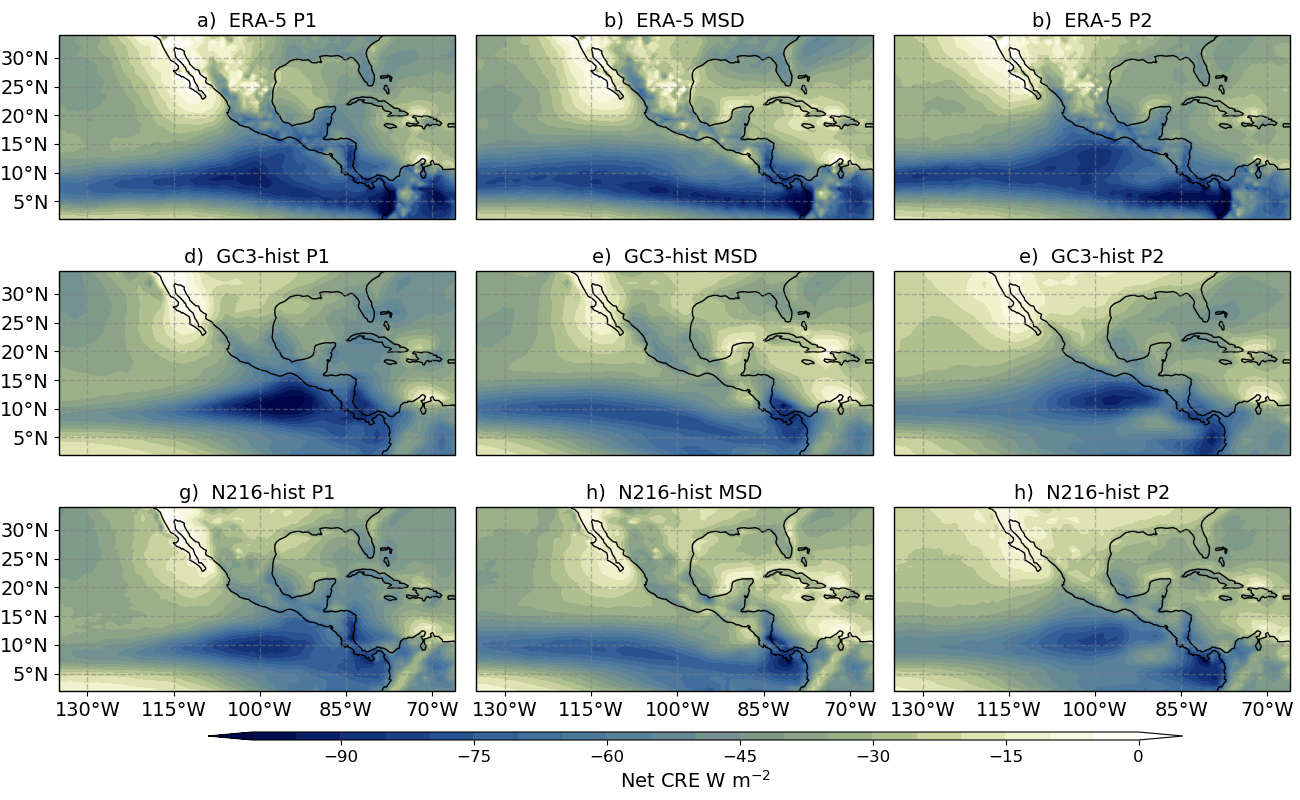
\includegraphics[width=\linewidth]{figures/fig4_creclim_3.png}
\caption[Composites of cloud radiative effects]{Composite mean cloud radiative effect (CRE) [W m$^{-2}$] during the periods of onset of the MSD, the MSD and the end of the MSD for (a-c) ERA5, and the ensemble mean of (d-f) GC3-hist and (g-h) N216-hist.}
\label{fig:cre_comp}
\end{figure}

\begin{multline}
CRE_{surf}=LW CRE_{surf} +SW CRE_{surf} \\ = LDS-LUS -(LDS_{cs}-LUS_{cs})+SDS-SUS-(SDS_{cs}-SUS_{cs}),
\end{multline}

\noindent where the fluxes are depicted as long-wave (L) or short-wave (S) and downwelling (D) or upwelling (U) at the surface (S) and the suscript $_{cs}$ denotes under clear-sky conditions. The long-wave upwelling at the surface (LUS) virtually cancels with the LUS$_{cs}$ because the long-wave emission from the surface is minimally dependent on the presence of clouds \citep{allan2011}. The net CRE at the surface is then given by:


\begin{equation}
CRE_{surf}=  LDS-LDS_{cs}+SDS-SUS-SDS_{cs}+SUS_{cs}.
\end{equation}



The net CRE during P1, MSD and P2 periods (Fig. \ref{fig:cre_comp}) is negative  and the minimum values are found in the East Pacific ITCZ region. The differences between the MSD timings closely follow the precipitation changes during these periods as the minimum CRE in the EP and the Mesoamerican region is found during the two peaks of precipitation with a weaker CRE over the Mesoamerican region and nearby basins during the MSD. The smallest CRE is found over the Baja California Peninsula. 
%During the MSD, the minimum in CRE is displaced west of the coastline into the region where the previous sections indicate increased convective activity.
The results of the two historical experiments closely follow the results of ERA5, and the only notable difference between the lower (GC3) and the higher (N216) resolution historical experiments is that the CRE is stronger in GC3-hist than in N216-hist.

\begin{figure}[t!]
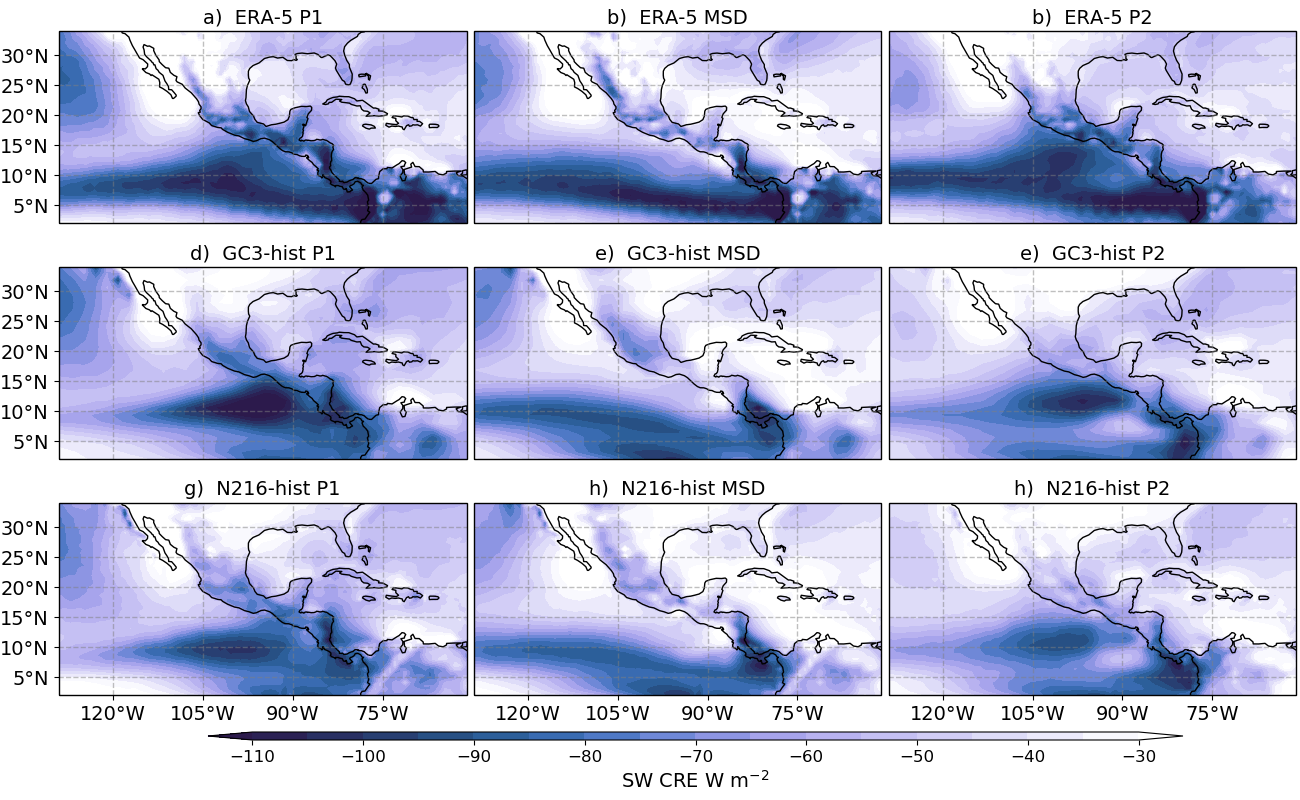
\includegraphics[width=\linewidth]{figures/fig4_swclim_3.png}
\caption[Short-wave cloud radiative effect composites]{As in Fig. \ref{fig:cre_comp} but for the short-wave radiative effect.}
\label{fig:sw_comp}
\end{figure}

The individual contributions of the SW and LW surface CREs (Figures \ref{fig:sw_comp} and \ref{fig:lw_comp}) show that the dominant term in the EP and Mesoamerican regions is the SW term. The negative SW CRE is strongest in the EP ITCZ region and the SW CRE varies with the MSD timings in similar fashion to the net CRE, i.e., in the MSD region, the SW term is notably larger ($<-90$ W m$^{-2}$) during the two peak periods of precipitation than during the MSD.
The historical experiments also show that the SW CRE is larger in magnitude in the EP ITCZ region and that the SW CRE over the MSD region varies notably in the three stages of the rainy season.

In contrast, the LW term (Figure \ref{fig:lw_comp}), is generally smaller in magnitude than the SW term and is largest over land and in the ocean west of the California. Over the EP and CSEA regions, the LW term shows very small horizontal gradients, indicative of a fairly horizontally homogenuous effect of clouds. 
The differences of the LW between the stages of the MSD are smaller than the SW term variations, but both in ERA5 and the simulations, the LW term over the EP and the Caribbean Sea is visibly larger during the two peak periods than during the MSD. 

\begin{figure}[t!]
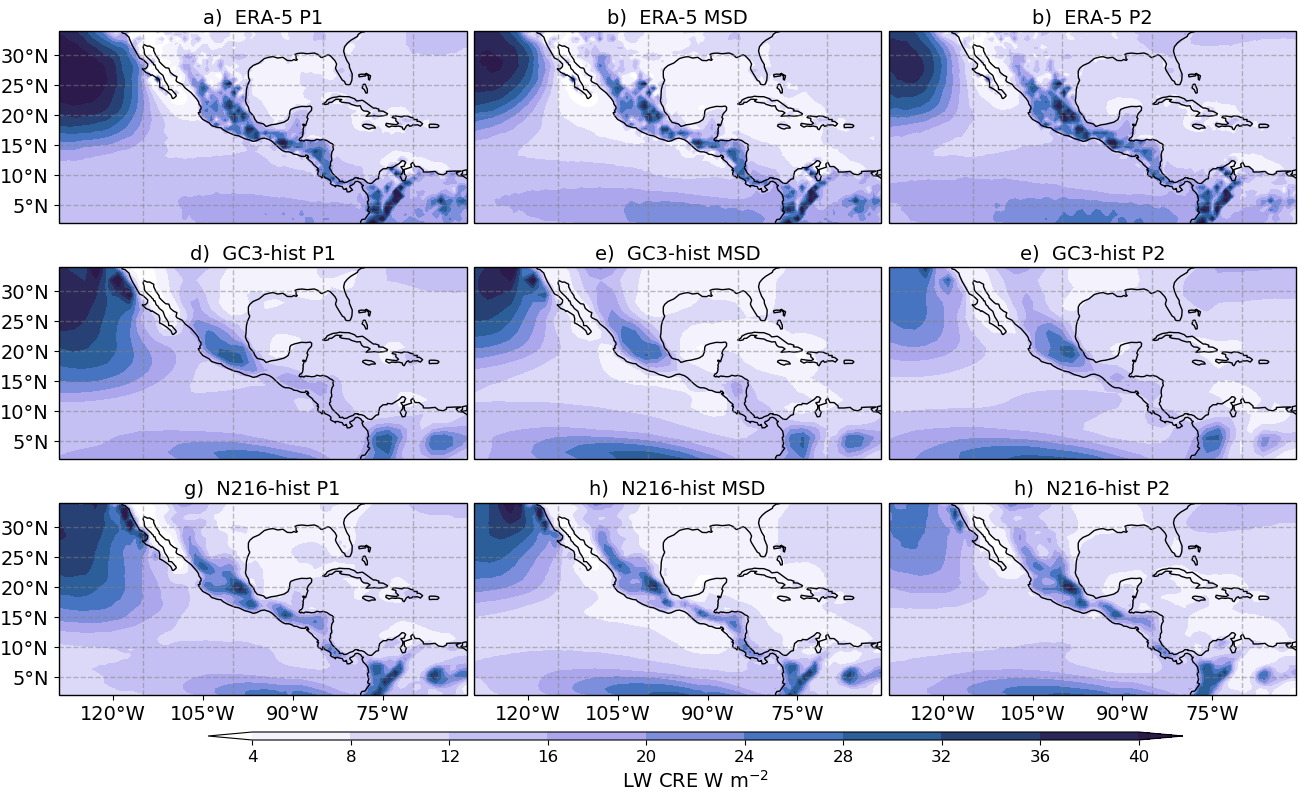
\includegraphics[width=\linewidth]{figures/fig4_lwclim_3.png}
\caption{As in Fig. \ref{fig:cre_comp} but for the long-wave CRE.}
\label{fig:lw_comp}
\end{figure}

These composites depict how the spatial distribution of the CRE varies with the MSD timings over the larger Intra-Americas Seas region, but how these terms actually within the season in the MSD region is not obvious. The seasonal cycles of the SW, LW and net CREs (Figure \ref{fig:cre_seasonal}a-c) show bimodal signals characterized by stronger CREs during the two peak periods during June and September and a relative minimum in between found in late July in ERA5 and early August in the simulations. The simulations reasonably simulate the magnitude of the net and SW CRE during the early summer season but overestimate the decrease in the net, SW and LW CRE during the midsummer, very likely associated with the underestimation of precipitation over this same period (Figure \ref{fig:msdcaribb}).

\begin{figure}[t!]
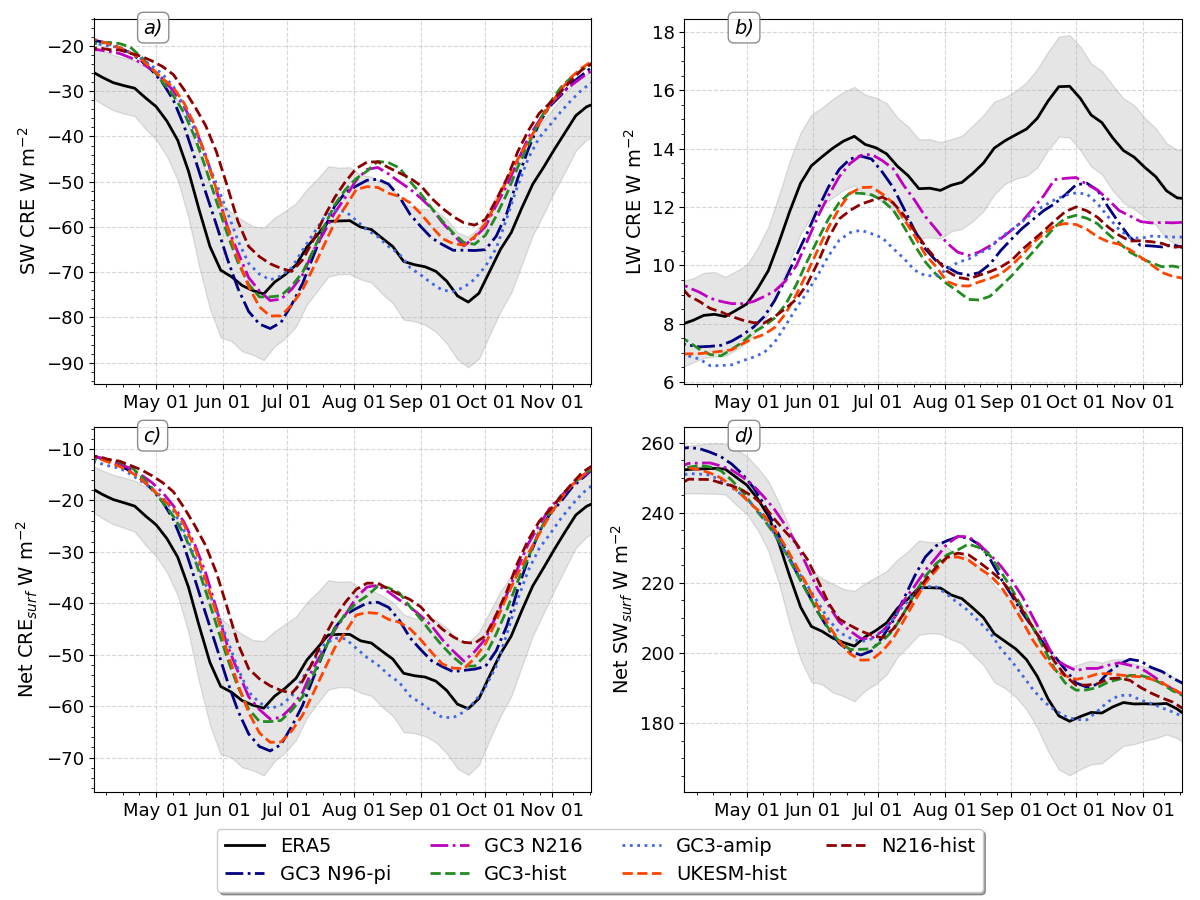
\includegraphics[width=\linewidth]{figures/cre_index_seasonal.png}
\caption[Seasonal cycle of cloud-radiative effects]{Pentad-mean seasonal cycle of the (a) SW and (b)  LW CREs, (c) the net CRE, and (d) the net SW at the surface, signed positive to indicate surface absorption of SW radiation.}
\label{fig:cre_seasonal}
\end{figure}

 Regardless of CREs, according to \cite{magana1999} and \cite{karnauskas2013}, the net SW (the difference between upwelling and downwelling shortwave) at the surface should also present a bimodal seasonal cycle.
In both ERA5 and the simulations, the net SW (Figure \ref{fig:cre_seasonal}d) follows a two-peak seasonal cycle characterized by a first peak in late May, which coincides with the peak in East Pacific SSTs. This peak in SW is followed by a local minimum during June which is followed by a secondary increase in July in ERA5 and extending to August in the simulations. After this second local maximum, there is another sharp decrease in the net SW at the surface at the end of the summer, which coincides with the the second peak in precipitation and therefore possibly linked with less downwelling SW. 

\begin{figure}[t!]
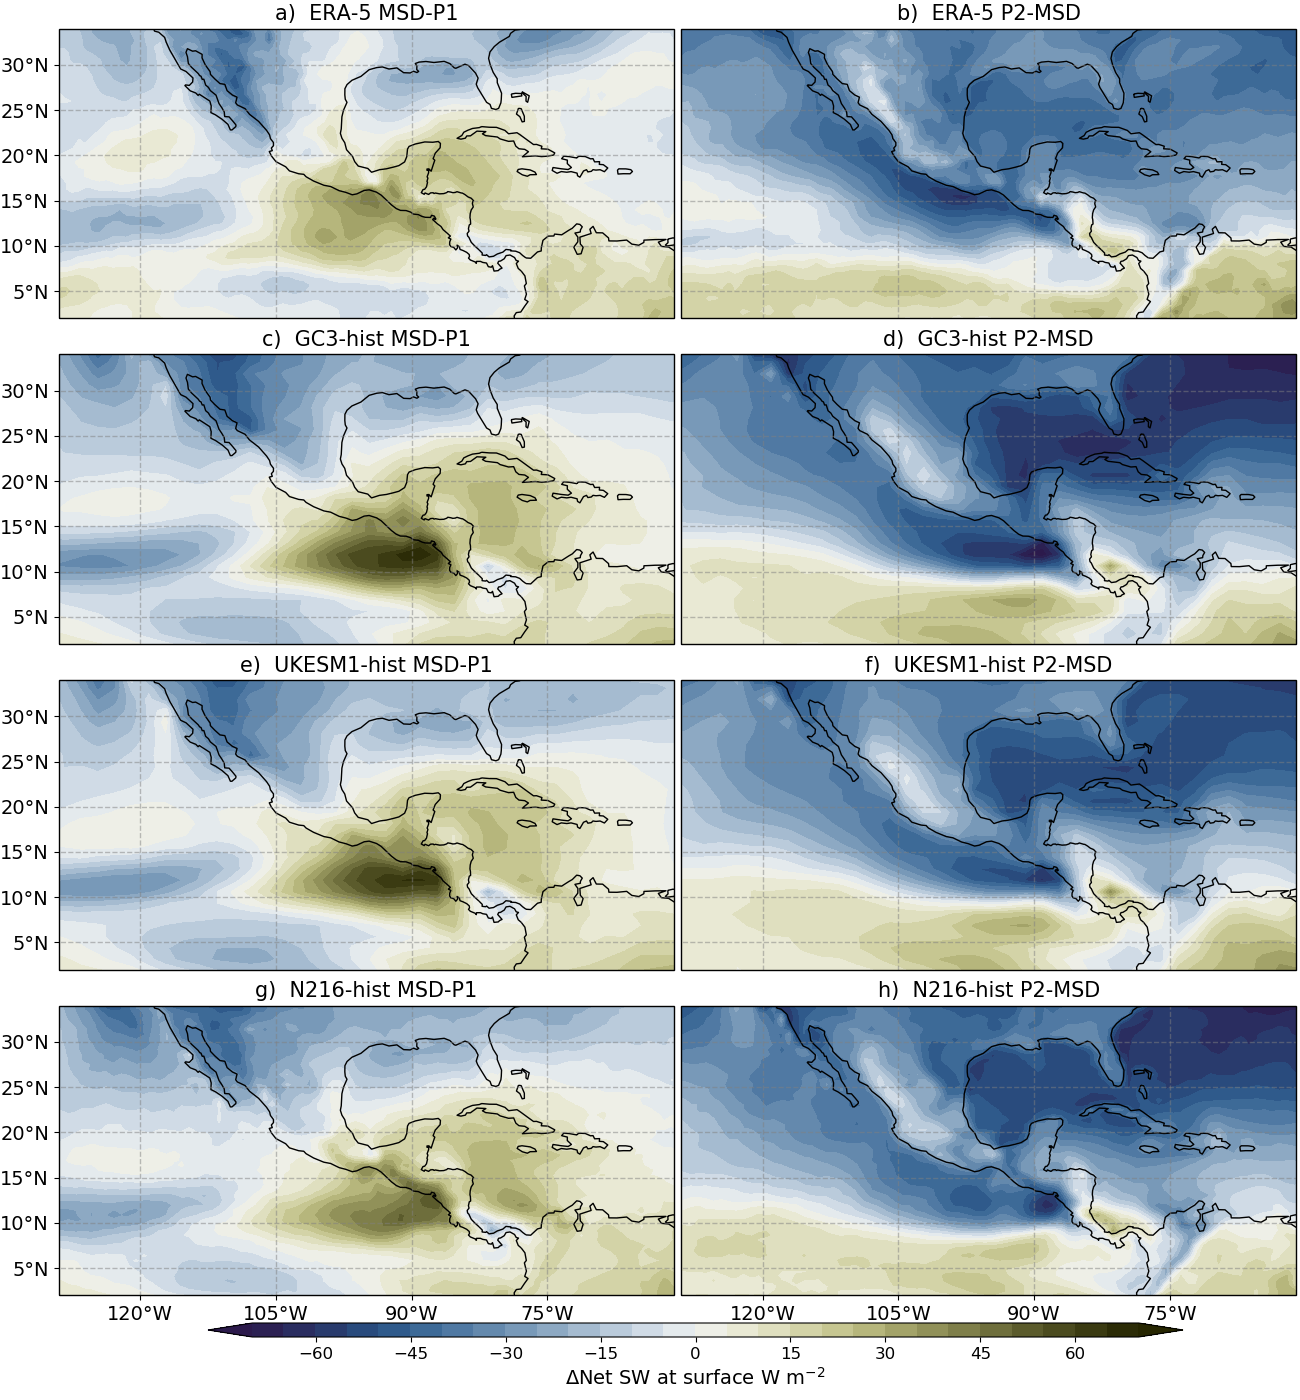
\includegraphics[width=\linewidth]{figures/fig4_netswdif_3.png}
\caption[Composite shortave differences with MSD timings]{As in Fig. \ref{fig:olranom}, but for the  net shortwave radiation [W m$^{-2}$] at the surface.}
\label{fig:swnet_diff}
\end{figure}

The spatial distribution of changes to the net SW at the surface (Figure \ref{fig:swnet_diff}) show that from the first peak to the MSD there is a positive difference net SW, indicative of more SW energy absorption at the surface of about 30 W m$^{-2}$ in ERA5 and 40 W m$^{-2}$ in the simulations. In contrast, for the P2-MSD differences, a notable reduction in net SW energy is observed throughout the North American continent but the maximum reduction is found on the western coast of southern Mexico. One might reasonably then suspect that the increased SW absorption during the MSD may indeed be a cause or part of the mechanism for the second peak of precipitation, as suggested by both \cite{magana1999} and \cite{karnauskas2013}. However, this could just be a correlation that highlights the coupling between clouds, radiation and precipitation and not necessarily that SW heating is the driving mechanism.

\begin{figure}[t!]
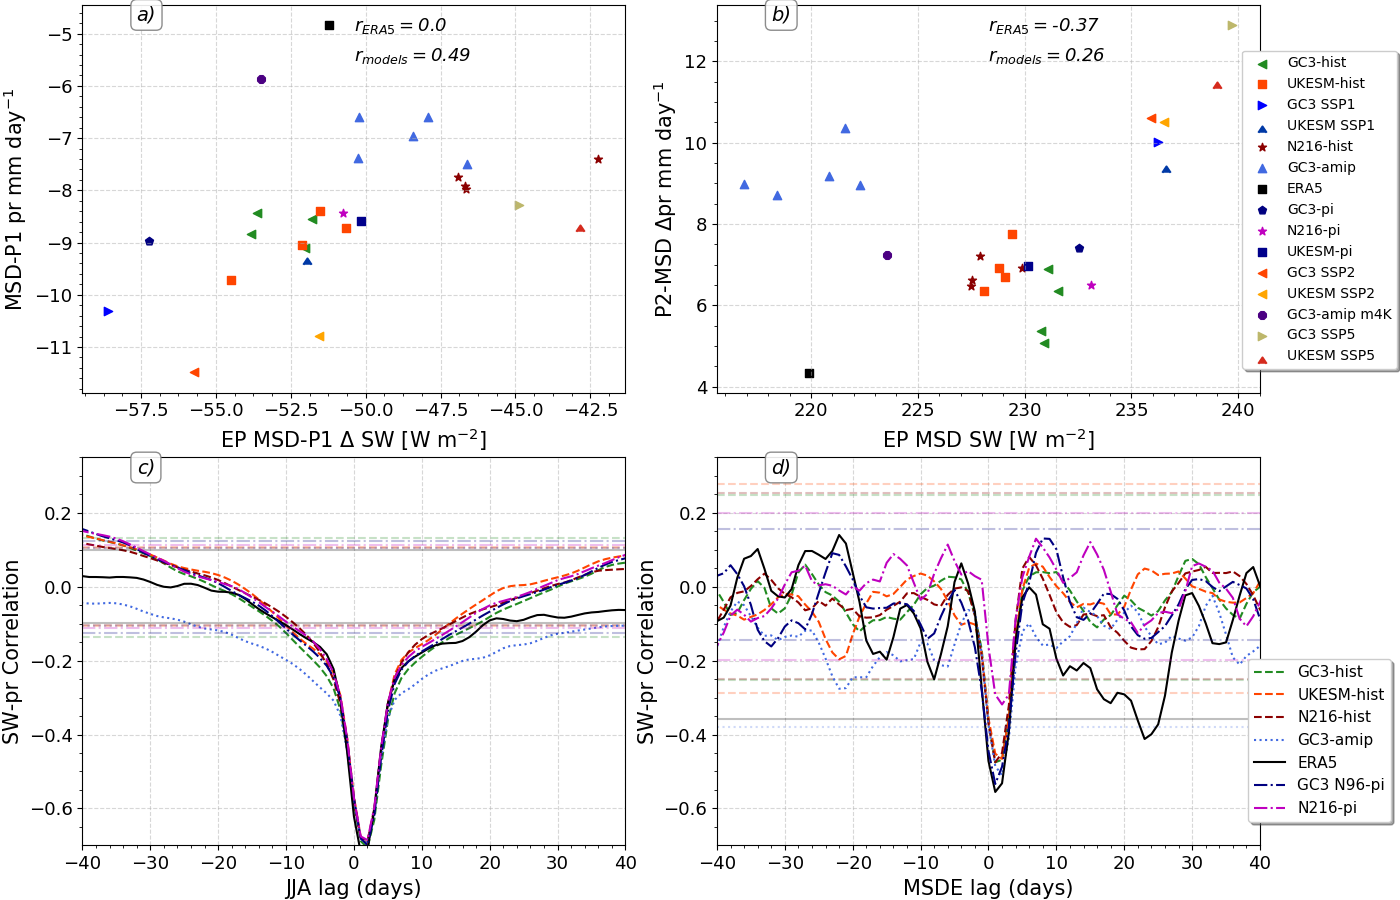
\includegraphics[width=\linewidth]{figures/cloud_scatter_f.png}
\caption[Scatterplot and lagged-regression of surface short-wave]{(a, b) Scatter of the mean changes to the net short-wave (SW) at the surface (abscissa) with respect to changes in precipitation for different MSD stages. (c, d) Lagged-regression coefficients between the net shortwave absorption in the East Pacific and precipitation over the MSD region for the (c) the JJA season and (d) around the MSDE date.}
\label{fig:cloud_scatter}
\end{figure}

These hypotheses are further tested through scatter and lag-lead regression analysis (Figure \ref{fig:cloud_scatter}). The changes to the net SW at the surface are unrelated to the interannual variability of the changes to precipitation in ERA5. The reduction in SW in the MSD-P1 periods shows a 0.0 correlation with the changes of precipitation during the same stages, whereas the net SW absorbed in the EP during the MSD period is negatively correlated with precipitation during the second peak. In other words, years where less shortwave is absorbed in the EP is associated with years stronger second peaks in the MSD region, in marked contrast to previous hypotheses. 

Furthermore, in the MOHC CMIP6 experiments there appears to be only a modest relationship between net SW and precipitation. The changes to SW during the MSD-P1 are only modestly related to precipitation as simulations that have the smallest changes to net SW in this period do not exhibit the smallest changes to precipitation. Similarly, a very weak relationship between SW and precipitation is found within the different experiments to relate the net SW at the surface during the MSD and the strength of the second peak. 

Lag-lead relationships (Figure \ref{fig:cloud_scatter}c, d) confirm that there is a strong correlation between SW and precipitation but this is a negative correlation at lag 0. This negative correlation illustrates that strong precipitation periods are associated with less shortwave absorbed by the surface, due to the high clouds blocking incoming SW. Correlations are not significant outside of lag -5 to 5 days near the MSDE date, although they appear significant for some coupled simulations at lags of -40 days when the entire JJA season is considered. These results appear contradictory with the argument of \cite{karnauskas2013} who argued a lagged relationship between shortwave absoprtion at the surface and precipitation at the end of the MSD. 


 
\begin{figure}[t!]
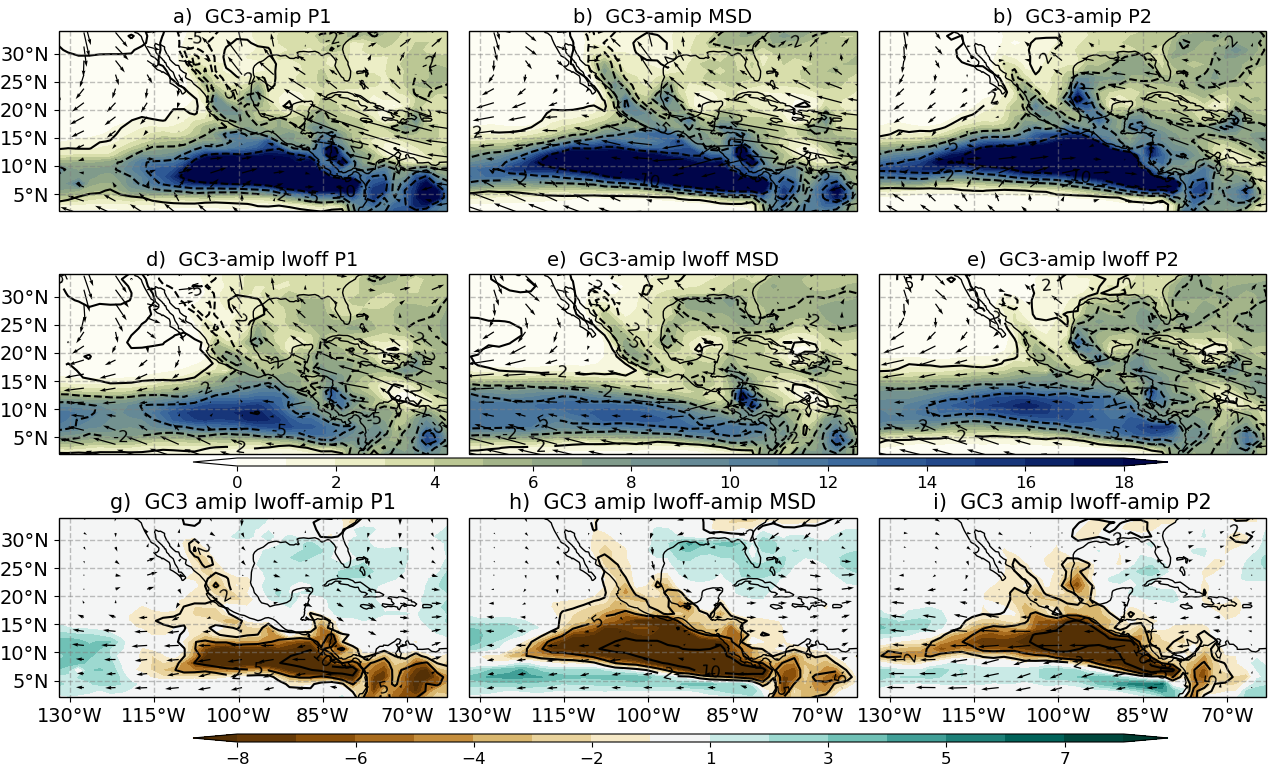
\includegraphics[width=\linewidth]{figures/lwfig_clim_1.png}
\caption[Composite moisture flux and wind speed]{Composite mean precipitation (shading in mm day$^{-1}$), vertical velocity (contours in 10$^{-2}$ Pa s$^{-1}$) and 850 hPa wind speed (vectors) for the P1, MSD and P2 periods in the (a-c) GC3-amip and (d-f) GC3-amip lwoff experiment. (g-i) shows the difference between the lwoff-amip and the amip experiments.}
\label{fig:lwoff}
\end{figure}

Finally, while the incoming SW radiation plays an important role in several theories for the MSD, the LW effects have important consequences in general monsoon dynamics \citep{guo2015,byrne2020}. 
The GC3-amip lwoff experiment is part of the contributions from the Cloud Feedback MIP (CFMIP)  \citep{webb2017} to CMIP6. This experiment is identical to the GC3-amip experiment except that the treatment of the LW in the radiation code in the model is not affected by the presence of clouds, in other words all LW fluxes are assumed to be under clear-sky conditions. 

The impact of the LW CRE for precipitation in the Mesomerican region is critical (Figure \ref{fig:lwoff}). When the LW effects of clouds are ignored, precipitation over the whole domain is greatly reduced (50-80\%), ascent becomes weaker and the low-level circulation also weakens. 
These results are in agreement with previous studies \citep{guo2015,byrne2020} that show that cloud radiative heating strengthens the local and regional circulation in a monsoon. The circulation and precipitation is so diminished in GC3 amip-lwoff that this is the driest simulation found in this chapter (Figure \ref{fig:scatter_msd}). The monsoon precipitation is so diminshed that small variations between the MSD and the two peak periods of precipitation are almost undistinguishable. 

This section diagnoses the seasonal cycle and spatial variability of CRE at the surface as depicted by ERA5 and the CMIP6 simulations. The net CRE at the surface is dominated by the SW term, indicating the strong effect that convective clouds have to block SW radiation from reaching the surface throughout the summer. The total absorbed SW shows a double-peak structure, with the second peak appearing at the end of the MSD period for both ERA5 and CMIP6 simulations, as suggested in the solar declination angle hypothesis \cite{karnauskas2013}. However, the strength and timing of the changes to the SW absorption suggest that the relationship between SW heating and precipitation is more of a correlation than a causal link from the SW to the precipitation. 



\section{The role of the Caribbean Low-Level Jet}



The previous sections evaluate the radiative-convective feedback and the solar declination angle hypotheses, in addition, this section examines the role of the Caribbean Low-Level Jet (CLLJ) for the MSD of Mesoamerica. Section \ref{sq:msdclim} shows that the seasonal cycle of the low-level zonal wind, i.e., the CLLJ, is well represented by the simulations (see Figure \ref{fig:csst}d), but the timing of the peak magnitude of the CLLJ in the models is delayed by about three weeks with respect to ERA5. The timing of the start of the MSD is notably also delayed in the models by around 10 days, according to Table \ref{tab:4} in the previous chapter. This evidence is suggestive that the CLLJ may be playing a role in the timings of the MSD in the simulations, which would be consistent with previous studies \citep[e.g.][]{herrera2015,martinez2019}.


The main dynamical argument that links the MSD in southern Mexico and Central America and the CLLJ is centred around variations in the moisture flux convergence (MFC), and subsequently in the total water content (TWC) \citep[see e.g.][]{gamble2008,herrera2015,martinez2019,zermeno2019}. For this reason, this section examines the CLLJ magnitude as measured by the 850 hPa zonal wind in the Caribbean Sea (see box in Figure \ref{fig:eof2}), and the integrated moisture flux convergence (IMFC) and TWC in the MSD region. 
The IMFC was calculated using the following equation from daily ERA5 data and daily data from the simulations:

\begin{equation}
IMFC=-\Bigg\langle \nabla \cdot \vec{u}q \Bigg \rangle
\label{eq:waterbudget}
\end{equation}

\noindent where $q$ is the specific humidity at each pressure level, $\vec{u}$ is the wind vector and $\nabla$ is the horizontal divergence operator and the $\langle \rangle$ operator denotes column integrals in the troposphere.


 \begin{figure}[t!]
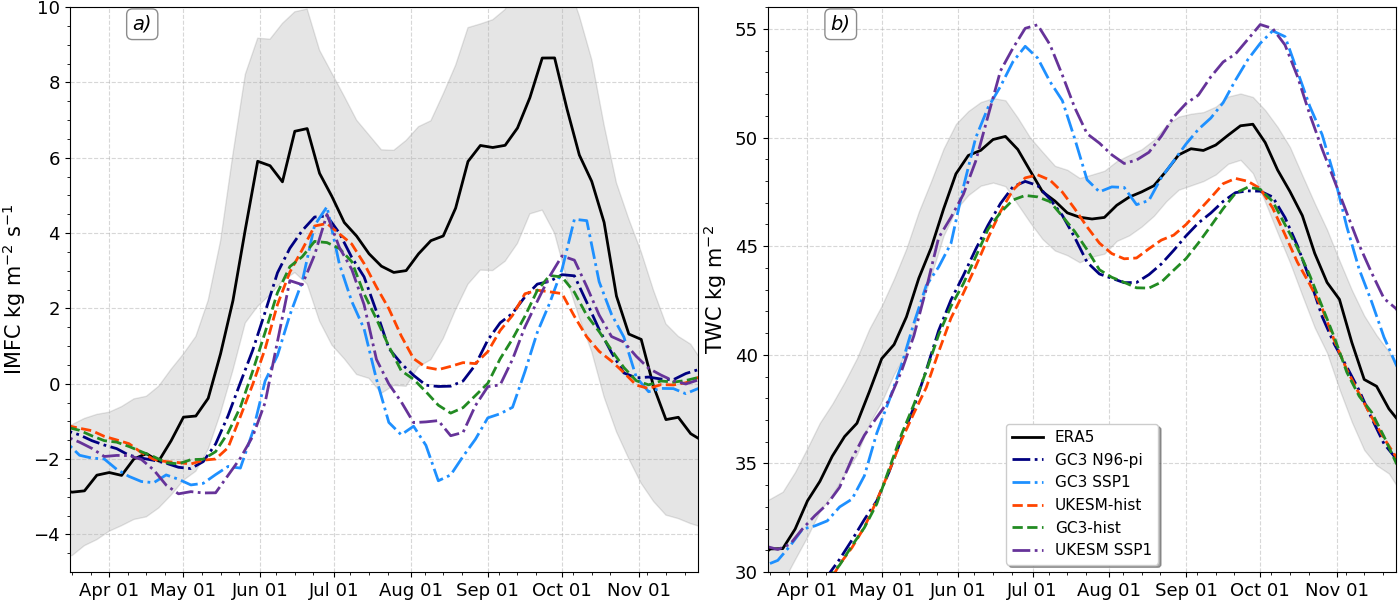
\includegraphics[width=\linewidth]{figures/imfd_index_seasonal}
\caption[Seasonal cycle of IMFC and TWC]{Seasonal cycle of (a) IMFC and (b) TWC averaged over the MSD region.}
\label{fig:imfd_cycle}
\end{figure}

The seasonal cycle of the IMFC and TWC (Figure \ref{fig:imfd_cycle}) averaged over the region of the MSD shows a strong bimodal signal, with two maxima in IMFC and TWC ocurring roughly at the same time as the two peaks in precipitation and a minimum found during Midsummer. The simulations follow closely the variations of the seasonal cycle of ERA5, but with a weaker IMFC over the region in all the simulations, particularly after the period of the first peak of precipitation. 

The magnitude of the two peaks of IMFC is fairly similar for all the simulations, in contrast with the asymmetry between the first and second peaks of precipitation, e.g., the historical experiments show a wetter first peak than the second peak. The IMFC during MSD, in contrast, shows notable differences amongst experiments, with the SSP1 experiments showing a smaller IMFC compared to the historical and piControl experiments, in fact in early August the IMFC is negative (indicative of moisture divergence) in the SSP1 experiments.


 The magnitude and timings of the two peaks in  TWC is fairly similar amongst the piControl and historical experiements and fairly similar to ERA5, however, notable differences exist. Firstly, the drying of the column in the simulations during midsummer occurs weeks after the drying in ERA5, which agrees with the differences in the seasonal cycle of precipitation. Secondly, the low-emission scenario (SSP1) runs show a higher TWC indicative of a moistening of the column throughout all the seasons for a relatively low greenhouse forcing. However,  the SSP1 experiments show the strongest decrease in TWC from the P1 to the MSD period of all the simulations, likely associated with the negative IMFC found during this period. Similarly, the SSP1 experiments show the strongest moistening of the column in late summer of all the simulations.

\begin{figure}[t!]
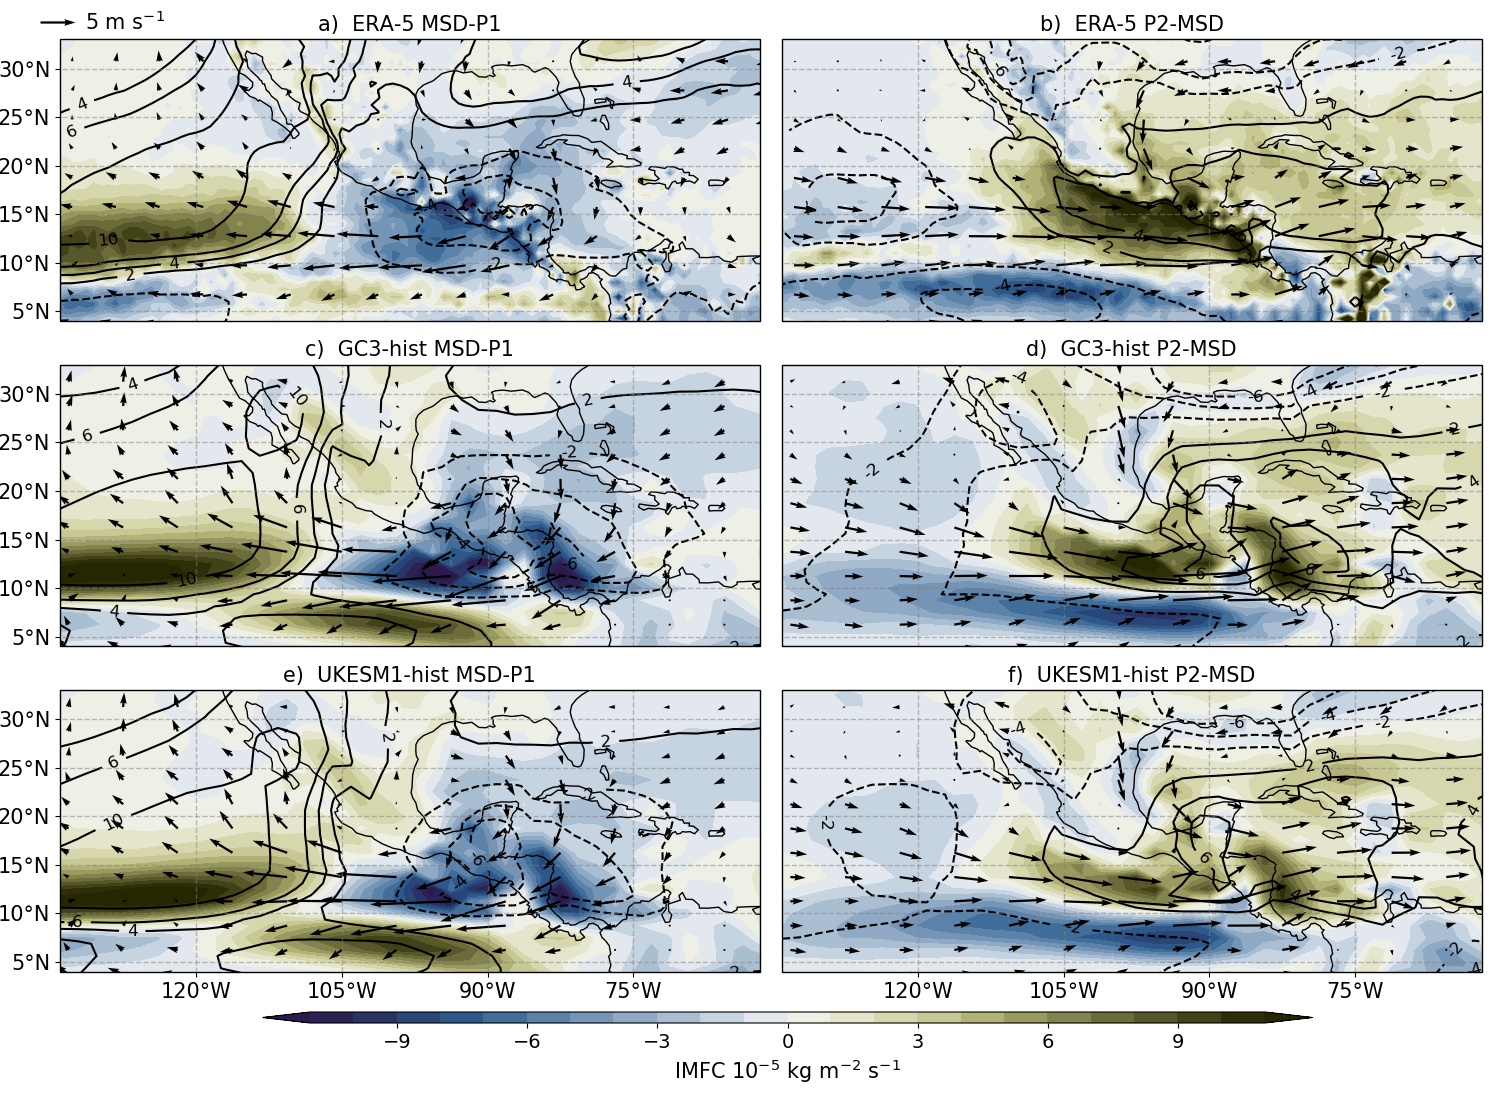
\includegraphics[width=\linewidth]{figures/imfdcomposite.png}
\caption[Composites of IMFC, TWC and CLLJ]{As in Figure \ref{fig:msdsstanom}, but showing variations in the IMFC (shading), TWC (contours in units of kg m$^{-2}$) and 850-hPa wind (vectors). }
\label{fig:msdmfcanom}
\end{figure}

The IMFC, TWC and 850-hPa wind variations associated with the MSD (MSD-P1 and P2-MSD) are shown in Figure \ref{fig:msdmfcanom} for ERA5 and two simulations. The patterns observed in the low-level wind vectors associated with the MSD timings follow closely the previously reported "MSD patterns" described by \cite{zermeno2019}, which confirms that the WT method is able to extract similar patterns in the low-level wind associated with the MSD to other techniques. 
The wind flow pattern in the MSD-P1 panel is characterised, both  in ERA5 and the simulations, by modest northeasterly anomalies in the Gulf of Mexico and the CSEA and strong easterly anomalies over the EP region. These wind anomalies indicate that as the wetter first peak period transitions to the drier MSD, the wind field changes from a weak low-level westerly wind to an easterly wind (see also Figure \ref{fig:csst}c). 
At the end of the MSD, the wind direction changes again to a westerly direction in the East Pacific, whereas the wind anomalies in the Caribbean Sea turn to westerlies indicative of a weakening of the CLLJ, coincident with the second peak of precipitation observed in the MSD region.

IMFC and TWC show coherent variations with the timings of the seasonal cycle of precipitation in the MSD region, with less moisture convergence and precipitable water in the column during the drier period compared to the two peak periods. 
 In contrast, west of the coast, at around the 125$^\circ$W, during the MSD there is increased TWC and IMFC in ERA5 and in the simulations, in agreement with the previous sections which showed increased convective activity in this region. Simultaneous to the drying of southern Mexico and Central America during the MSD, the North American monsoon region moistens as shown by the increased TWC and IMFC. 

 \begin{figure}[t!]
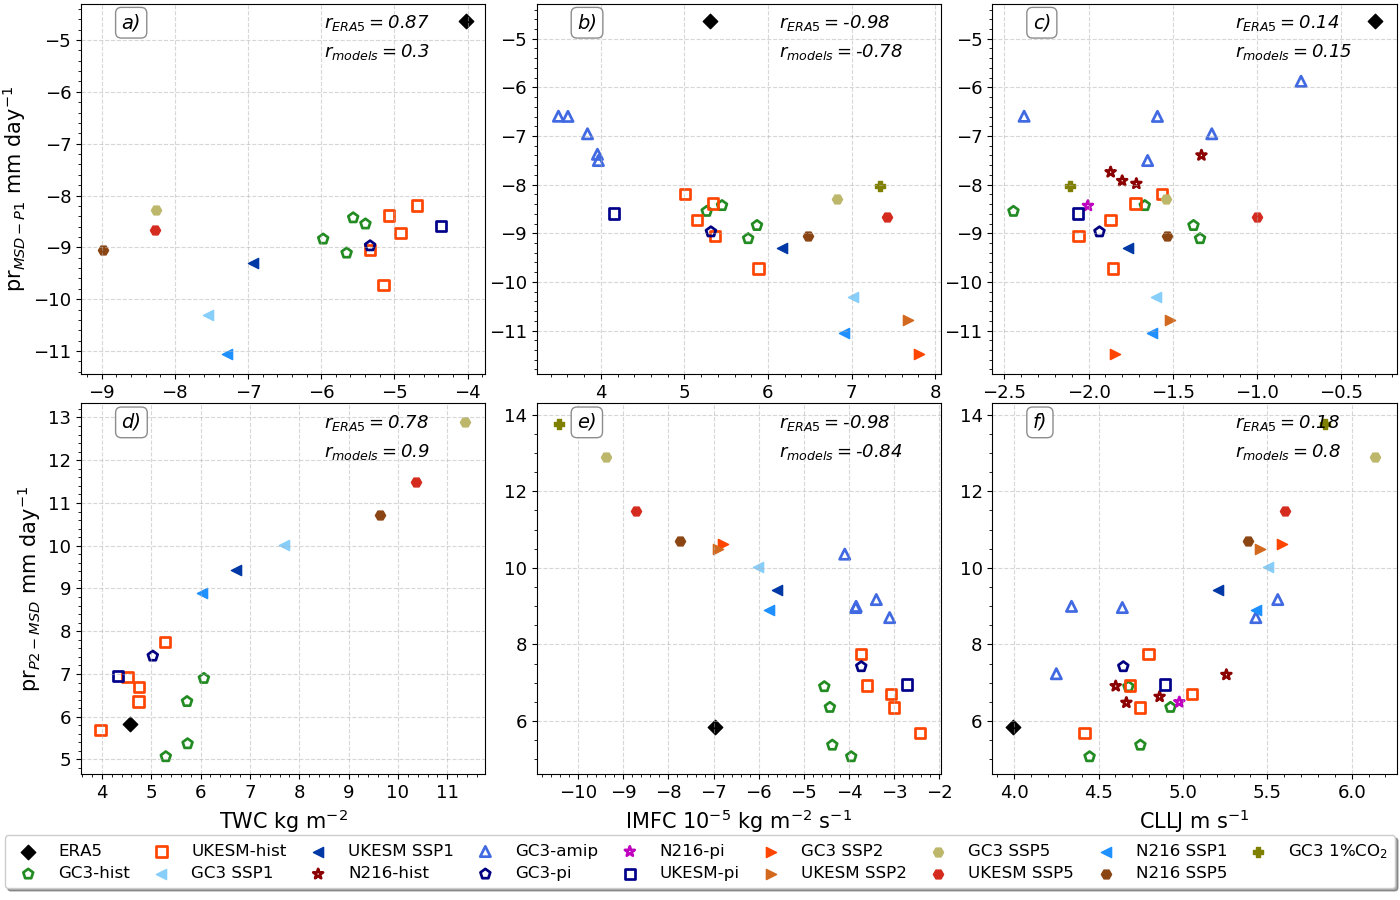
\includegraphics[width=\linewidth]{figures/imfd_scatter}
\caption[Scatterplot of TWC, IMFD and CLLJ]{As in Figure \ref{fig:var_sst_lhf_scatter}, showing the scatter of mean changes (a-c) MSD-P1 and (d-f) P2-MSD periods, but using the (a, d) IMFD and (b, e) TWC in the MSD region and the (c, f) CLLJ on the x-axis and precipitation in the MSD region in the y-axis.  }
\label{fig:imfd_scatter}
\end{figure}


In turn, the IMFC and TWC anomalies associated with the end of the MSD period, depicted by the P2-MSD panel,  show positive differences in the MSD region and negative anomalies southward, suggesting increased IMFC and TWC over southern Mexico and northern Central America, in agreement with the secondary increase in precipitation. Positive TWC and IMFC differences extend from the MSD region to the east into Cuba, the Caribbean Sea and the Gulf of Mexico. This moistening coincides with increased moisture divergence to the south of the MSD region in the East Pacific (120-90$^\circ$W,3-10$^\circ$N) and decreased TWC. 

%These composite results indicate that the changes to the precipitation in the MSD region are associated with moistening/drying of the column and changes to the horizontal convergence of moisture. 

Furthermore, a scatter plot of the mean changes to the IMFD, TWC and the CLLJ and their relationship to the syncrhonous variations in precipitation (Figure \ref{fig:imfd_scatter}) confirm that these diagnostics are deeply related to the timings and strength of the three stages in the seasonal cycle of precipitation. The interannual variability of the precipitation differences between the first peak and the MSD periods in ERA5  are very well explained by the interannual variability of the TWC ($r=0.87$) and the IMFC ($r=-0.98$) but less so by the CLLJ ($r=0.14$). The inter-experiment variability in the MSD-P1 precipitation differences can largely be explained by the inter-experiment differences in IMFC changes during the MSD-P1 periods ($r=0.78$). However, the changes in the CLLJ and IMFC in the simulations can not explain the precipitation differences between the runs in the MSD-P1 panels. 

\begin{figure}[t!]
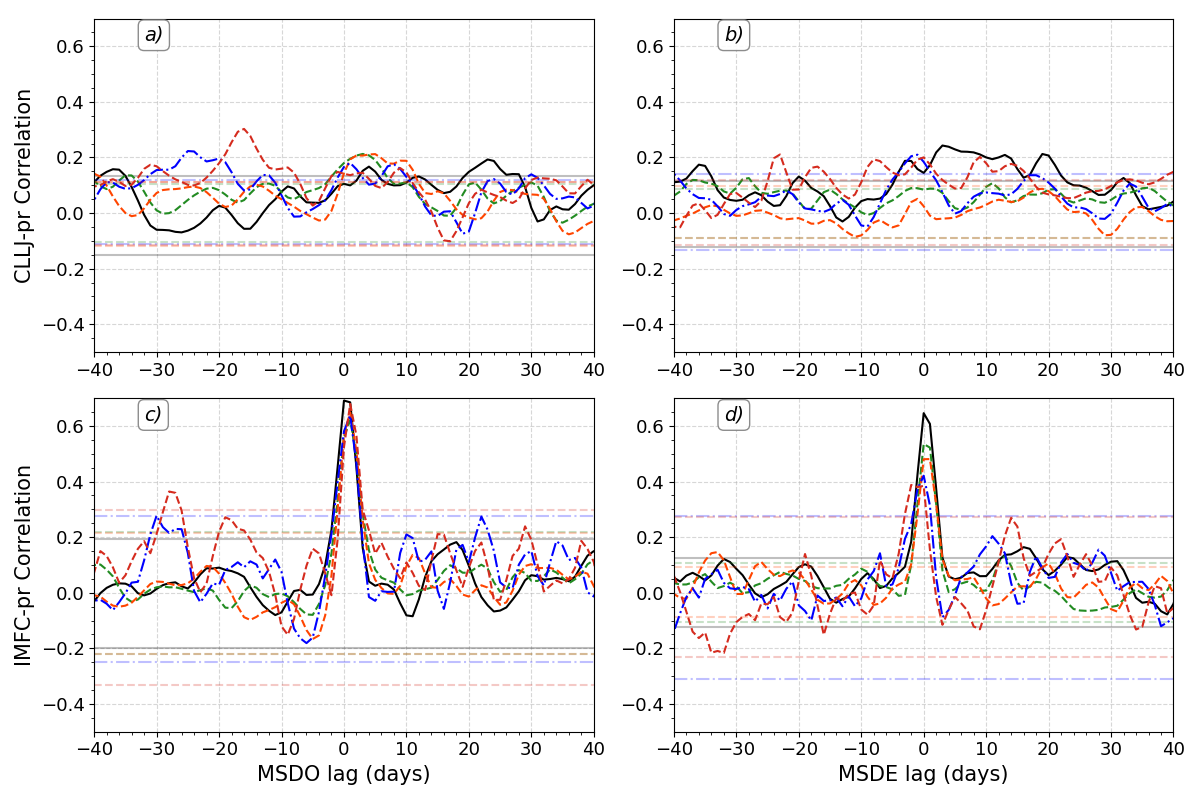
\includegraphics[width=\linewidth]{figures/lag_imfdcllj.png}
\caption[Lagged correlations of the CLLJ and IMFC indices with precipitation.]{Lagged correlations between precipitation in the MSD and the (a, b) CLLJ, defined as the 925 hPa zonal wind averaged over the CSEA region, and (c, d) the IMFC over the MSD region. Correlations are shown with lags computed with respect to the (a, c) onset and (b, d) end dates.  }
\label{fig:cllj_lag}
\end{figure}



The changes from the MSD to the second peak of precipitation (lower row in Figure \ref{fig:imfd_scatter}) in the simulations are very well explained by the mean variations to the CLLJ, the TWC and the IMFC. However, for the interannual variability of ERA5, only changes to the TWC and IMFC show significant and relatively high correlations. These results would suggest that variability in the CLLJ can explain several differences in the magnitude of the P2-MSD differences in the models, possibly through the modulation of the CLLJ on the TWC and the IMFD over the continent; nevertheless, the observed interannual variability of the CLLJ cannot explain the interannual variability in the strength of the second peak. %but the same argument does not apply to ERA5. 

The synchronous relationship found in the previous scatterplot is further tested via lagged correlations, shown in Figure \ref{fig:cllj_lag}. These correlations do not show any evidence that the nature of the relationship between the CLLJ or the IMFC with precipitation over the MSD is of a lagged nature. In particular, the correlations of precipitation with the CLLJ are not higher than 0.3 at any lag and only become significant for a few days in some simulations. In particular, around the MSDE date, no correlation at negative lags is notably positive or significant which is at odds with the hypothesis that CLLJ is responsible for the end of the MSD. 

However, the strength of the CLLJ may not be the relevant factor, but rather the influence of the CLLJ on the IMFC. The correlation of IMFC with precipitation shows a strong positive correlation, both at MSDO and MSDE in reanalysis and models around lag 0, and similar results are found for TWC-pr correlations (not shown). However, there is little evidence that this relationship is of a lagged nature, as the correlations are not significant far away from the 0 lag. 



\section{A short look at the MSD through the lense of the moist static energy budget}

The previous sections have tested three leading hypothesis for the Midsummer drought, with results suggesting that only elements of the CLLJ hypothesis can explain the interannual variability in the strength of the MSD in reanalysis, as well as in the differences between the CMIP6 experiments. However, changes to the CLLJ and IMFC appear to be unrelated to the strength and time of the onset of the MSD, which means that other processes are responsible for the start of the drier MSD period. 
To further explore the processes that control the start of the MSD, the moist static energy (MSE) budget is used in this section to disentagle how the column MSE budget terms vary over the wet season.

\begin{figure}[t!]
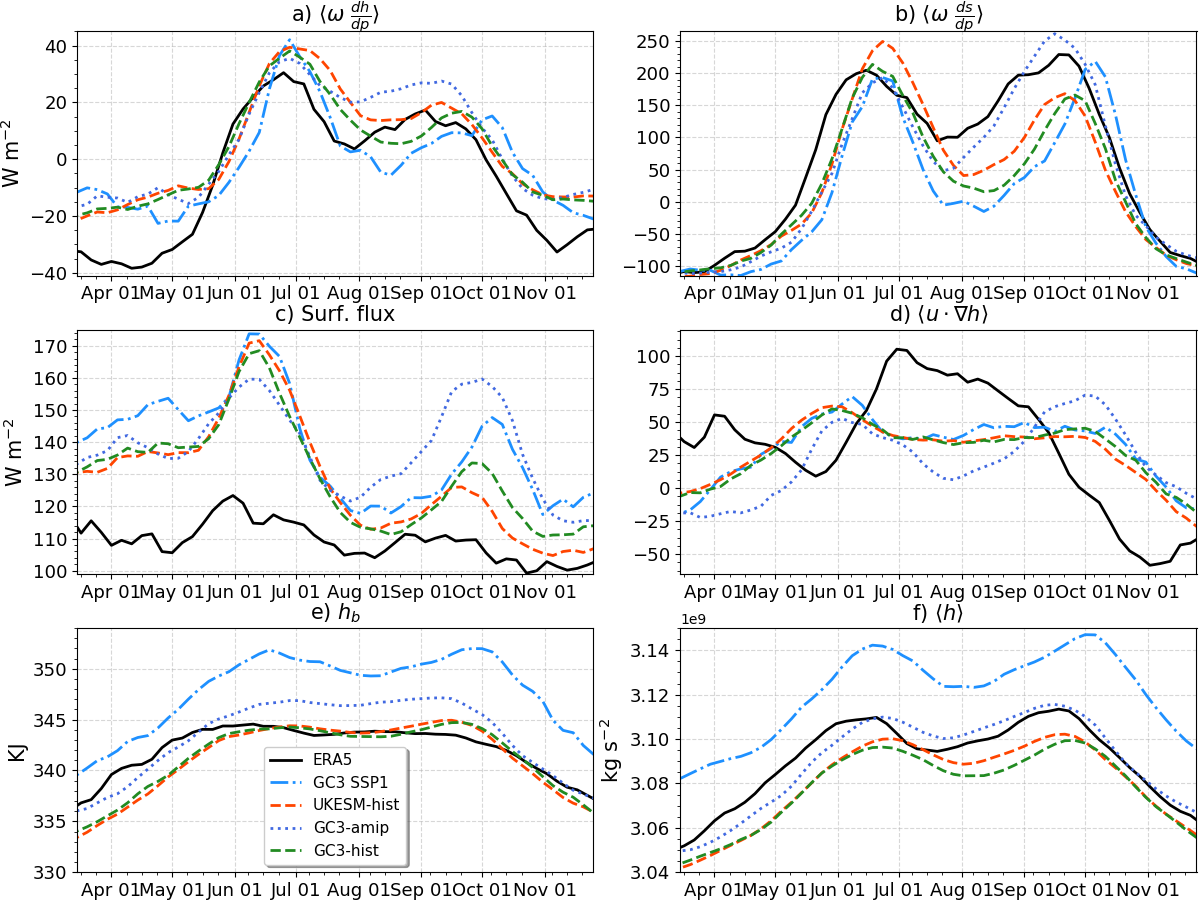
\includegraphics[width=\linewidth]{figures/thermopentad}
\caption[Seasonal cycle of MSE budget terms]{Pentad-mean seasonal cycle of the moist static energy budget terms. Vertical advection of (a) moist and (b) dry static energy, (c) the sum of the latent and sensible heat fluxes, (d) horizontal advection of MSE, (e) boundary layer MSE ($h_b$) and total column MSE ($\langle h \rangle$). The quantities in panels c,d were averaged over the EP region and the rest of the panels over the MSD region. }. 
\label{fig:thermo_pentad}
\end{figure}

 %The purpose of this section is not provide a new theory for the MSD but rather to show whether the investigation of the MSD through the lense of the MSE budget may prove more promising to understand these mechanisms than traditional theories and diagnostics. 


 The computation of the MSE budget terms is done as described in section \ref{sq:msemethod}. The budget terms are obtained from daily-mean values at all available levels within the troposphere for reanalysis and climate model output. It should be noted that the radiative heating terms are not available from the CMIP archive on daily scales so a full budget was not feasible with model data. In turn, we focus on the vertical and horizontal advection of MSE, the total column MSE, the surface fluxes and the gross moist stability.
 
  First, the seasonal cycle of the column budget terms, as well as the boundary layer or near surface MSE ($h_b$), is shown in Figure \ref{fig:thermo_pentad} with some quantities shown for the EP region and others for the MSD region. The vertical advection of dry ($s$) and moist ($h$) static energy shows a clear bimodal seasonal cycle, with two peaks at the start and end of the summer season, separated by a local minimum that occurs at the end of July or early August.
 The simulated vertical advection of MSE corresponds well with ERA5 during the wet season (JAS) for all the simulations, although the vertical advection of $s$ is smaller in the historical and SSP1 experiments during the MSD and second peak periods. The vertical advection of $s$ is not underestimated by the GC3 amip experiment during late summer, which has a wetter second peak as shown in previous sections. 

\begin{figure}[t!]
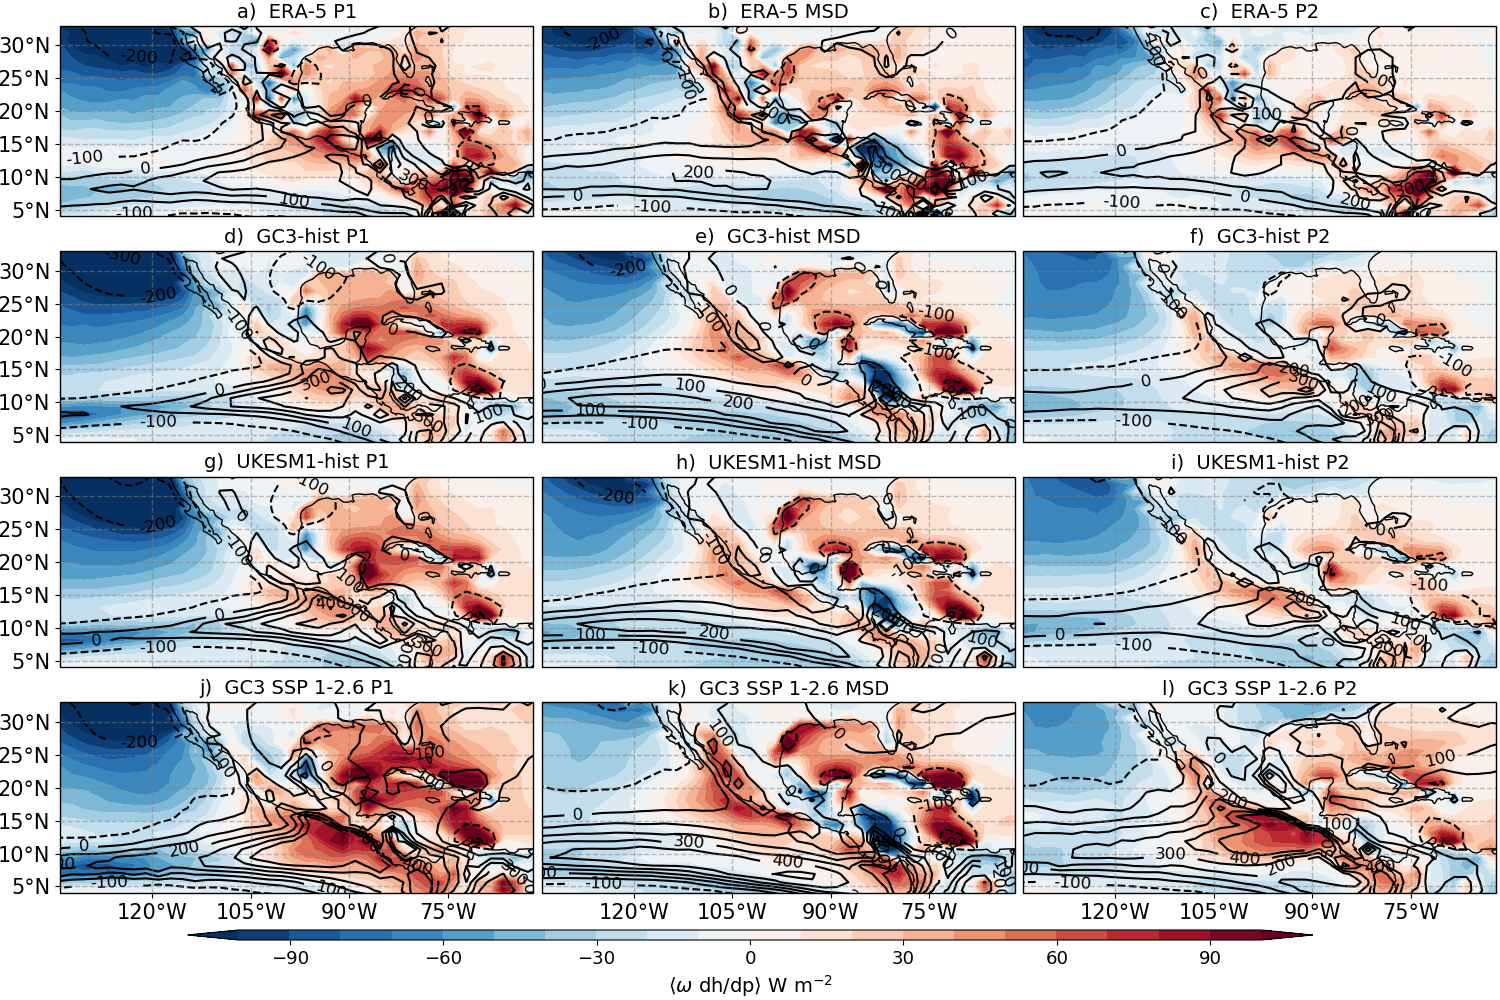
\includegraphics[width=\linewidth]{figures/thermocompositewdhdp.png}
\caption[Composites of the mean vertical advection of the MSE budget]{Composites of mean $\langle \omega dh/dp \rangle$ (shading in W m$^{-2}$) and $\langle \omega ds/dp \rangle$ (contours in W m$^{-2}$).  }
\label{fig:wdhdpcompo}
\end{figure}  
 
 The sum of the latent and sensible heat fluxes in the EP region show a clear bimodal signal in the experiments but not in ERA5. The experiments also show very large biases during both periods of peak precipitation in June and Sep-Oct. In late summer, this bias is particularly notable in the GC3 amip experiment. These biases in the surface fluxes in the EP are arguably one of the reasons for the very wet bias found in the EP ITCZ in these models. 
 
\begin{figure}[t!]
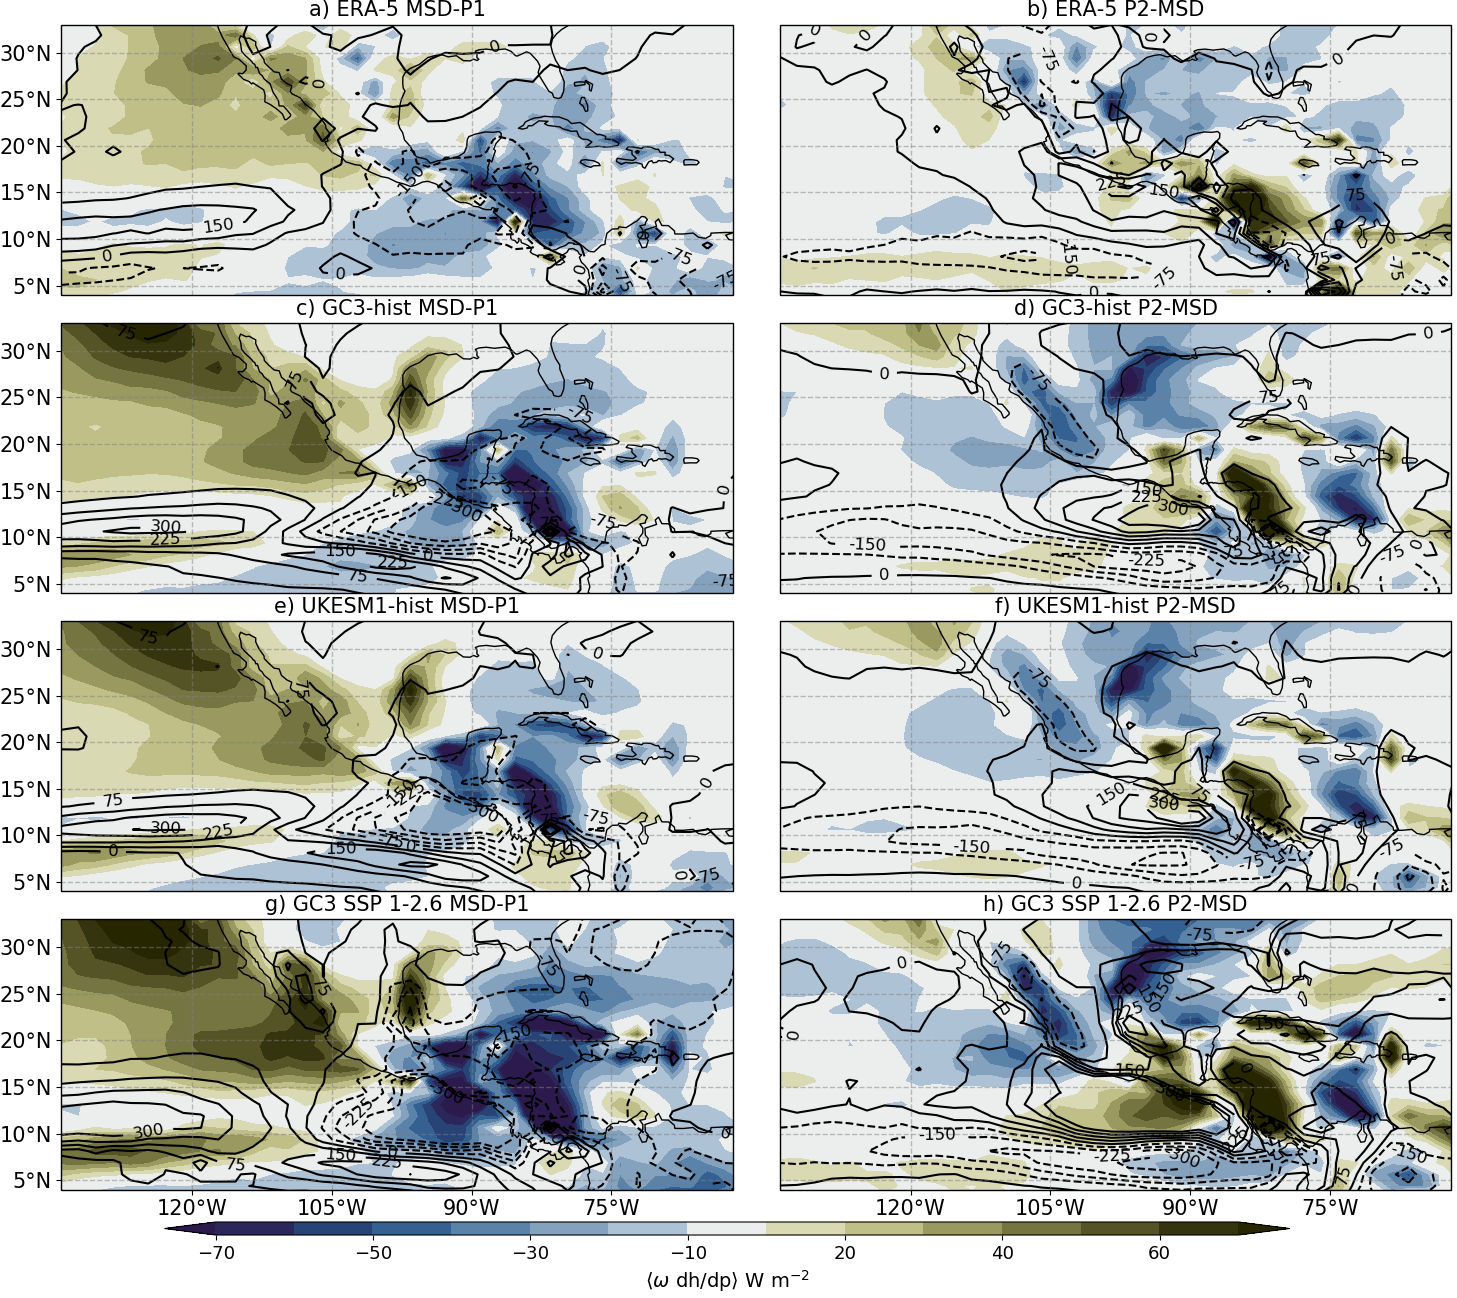
\includegraphics[width=\linewidth]{figures/thermocompositewdhdpanom.png}
\caption[Composites of the anomalous vertical advection of the MSE budget]{Composites of the differences (a, c, e, g) MSD-P1 and (b, d, f, h) P2-MSD of $\langle \omega dh/dp \rangle$ (shading in W m$^{-2}$) and $\langle \omega ds/dp \rangle$ (contours in W m$^{-2}$).  }
\label{fig:wdhdpanom}
\end{figure} 
 

One component of the theory by \cite{karnauskas2013} involved the net shortwave part of the surface energy balance being notably different during the various stages of the MSD. A direct implication from this hypothesis is that the shortwave ultimately influences the surface or boundary layer MSE (Fig. \ref{fig:thermo_pentad}e). However, in most of the simulations and ERA5, $h_b$ in the MSD region follows a plateau-like seasonal cycle with a clear increase during spring, a plateau during summer and a sharp decrease in October at the end of the rainy season. The SSP1 experiment shows a  decrease in $h_b$ in August but this is fairly modest compared to the magnitude of the change in $h_b$ at the end and start of the summer. 

Similarly, the total column $h$ shows a modest bimodal seasonality in reanalysis and simulations, i.e., $\langle h \rangle$ decreases at the midsummer. 
The low-emission scenario shows a notable increase in total column $h$ compared to historical and pre-industrial experiments, and higher emission scenarios (SSP2 and SSP5) showed that total $h$ scales with greenhouse forcing (not shown). One key aspect of this increase in total column $h$ is that total precipitation is not increased uniformly over all the stages of the wet season (see Fig. \ref{fig:scatter_msd}). 

The spatial distribution of the mean $\langle \omega dh/dp \rangle$ and $\langle \omega ds/dp \rangle$ (Figure \ref{fig:wdhdpcompo}) during the three stages of the MSD seasonal cycle show a good agreement between the experiments and reanalysis. The highest values of $\langle \omega ds/dp \rangle$ are found on the western coast of northern Central America, in the easternmost position of the ITCZ. Positive values of $\langle \omega dh/dp \rangle$  are found in the Caribbean Sea, the Gulf of Mexico and over the Mesoamerican region throughout the three stages of the MSD. Negative values of $\langle \omega dh/dp \rangle$ and $\langle \omega ds/dp \rangle$ are found over the coast of California throughout the wet season. 

\begin{figure}[t!]
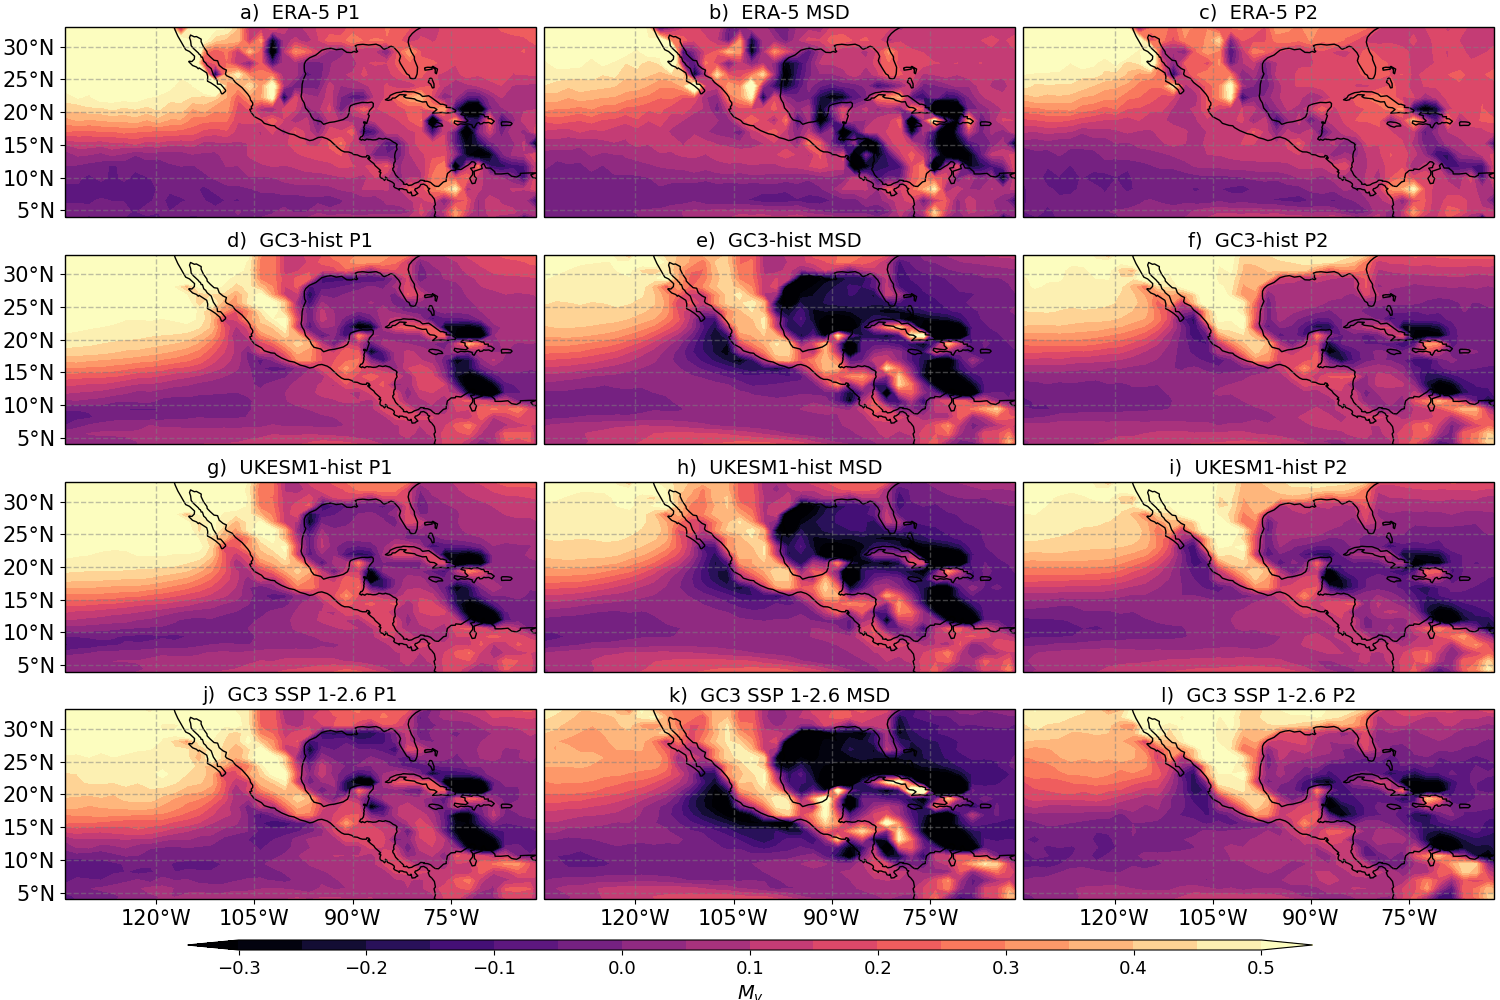
\includegraphics[width=\linewidth]{figures/thermocompositeMvclim.png}
\caption[Composites of gross moist stability]{Composites of vertical gross moist stability ($M_v$) in the three stages of the Midsummer drought for ERA5 and three experiments.  }
\label{fig:Mvcompo}
\end{figure} 
 
 The changes to the $\langle \omega dh/dp \rangle$ and $\langle \omega ds/dp \rangle$ during the MSD periods are best illustrated in Figure \ref{fig:wdhdpanom}, which shows the differences between MSD-P1 and P2-MSD. In the Mesoamerican region, $\langle \omega dh/dp \rangle$ and $\langle \omega ds/dp \rangle$ are reduced during the MSD period compared the first peak period, this difference is maximized right at the exit of the Gulf of Tehuantepec, in southwestern Mexico. 
 Simultaneously, from the P1 to the MSD period, $\langle \omega ds/dp \rangle$ notably increases west of the Mesoamerican region near the 125$^\circ$W region whereas $\langle \omega dh/dp \rangle$ increases in northern Mexico and in the Gulf of California. 
 
\begin{figure}[t!]
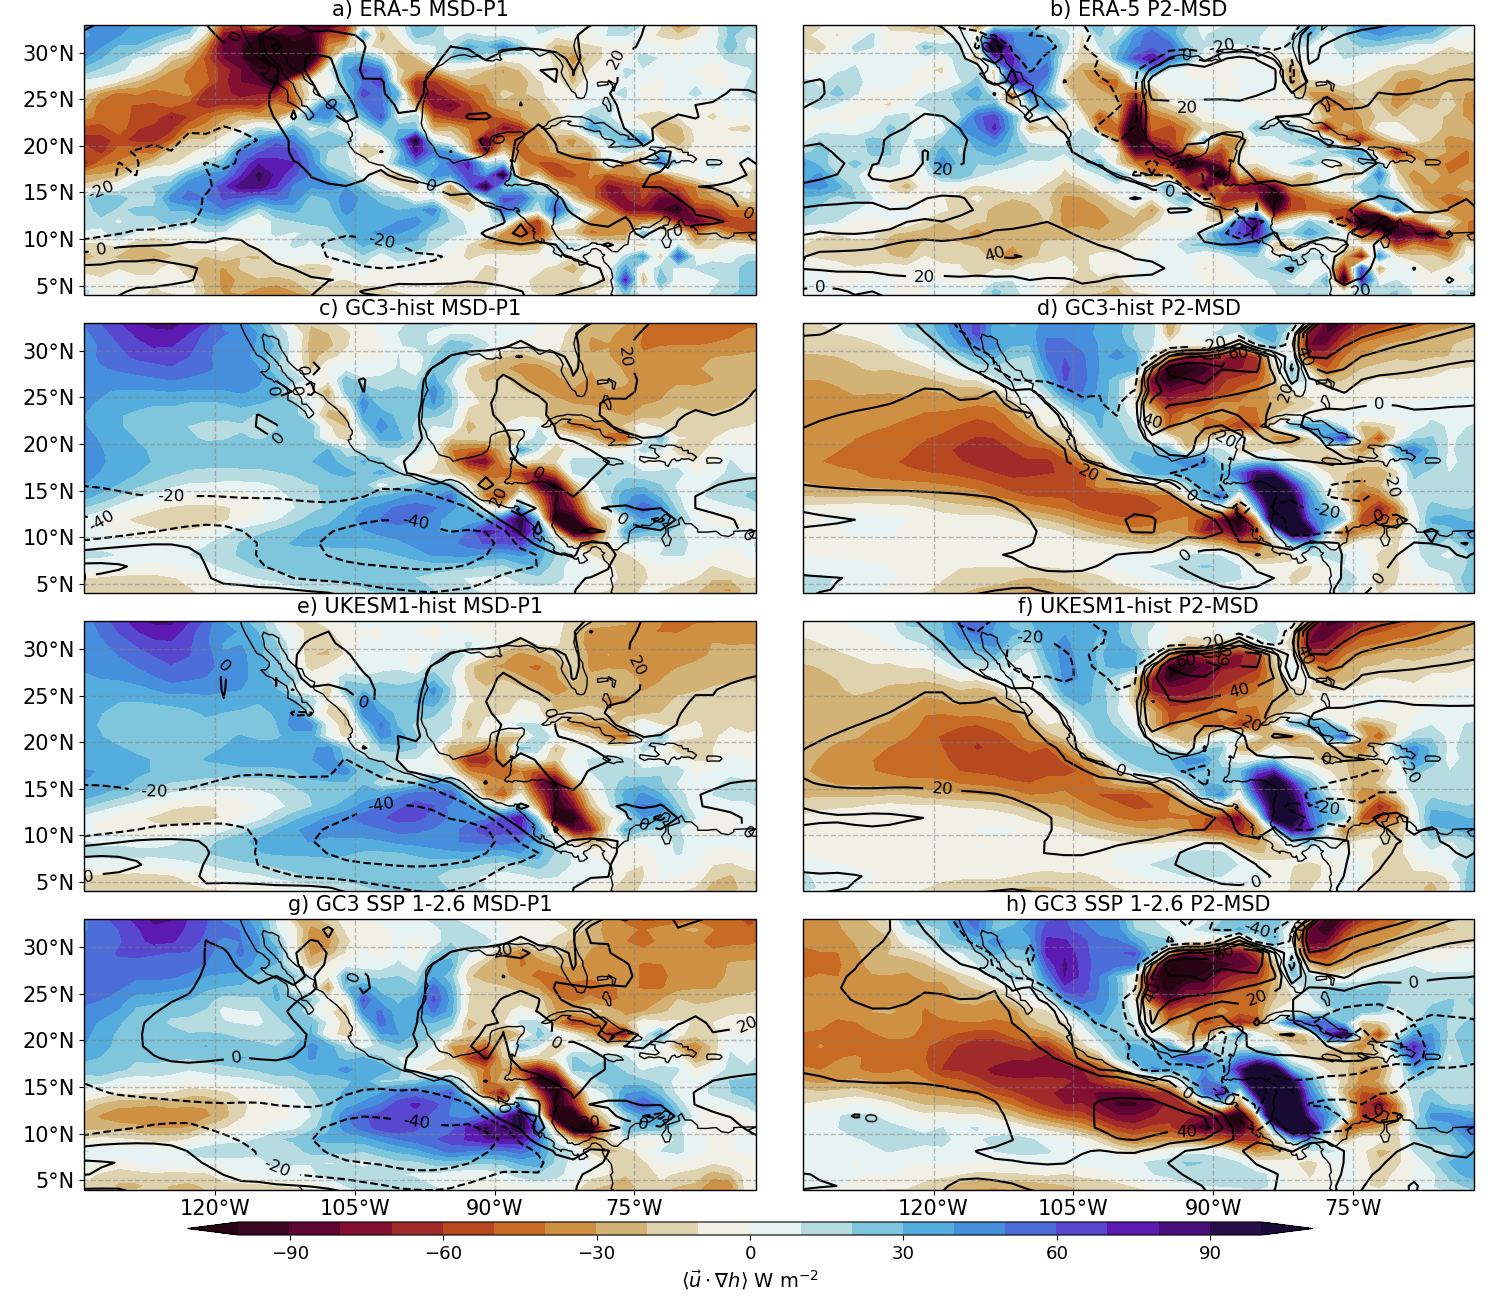
\includegraphics[width=\linewidth]{figures/thermocompositeint_udothanom.png}
\caption[Composites of the anomalous horizontal advection of MSE and surface fluxes]{Composites of the differences (a, c, e, g) MSD-P1 and (b, d, f, h) P2-MSD of $\langle \vec{u}\cdot\nabla h \rangle$ (shading in W m$^{-2}$) and total surface fluxes ($F$) (contours in W m$^{-2}$).  }
\label{fig:intudothanom}
\end{figure} 
  
 
 At the end of the MSD, illustrated by the P2-MSD panels in Figure \ref{fig:wdhdpanom}, $\langle \omega dh/dp \rangle$ and $\langle \omega ds/dp \rangle$ increase notably in the Mesoamerican region. Again, the maximum difference of $\langle \omega ds/dp \rangle$ is found in the Gulf of Tehuantepec region. The North American monsoon region show a decrease in both $\langle \omega dh/dp \rangle$ and $\langle \omega ds/dp \rangle$. 
 Both for the P2-MSD and MSD-P1 panels, the experiments are able to reproduce the spatial patterns of these changes to these budget terms. Furthermore, the SSP1 experiment shows larger differences between the MSD stages compared to the historical experiments.

The normalized gross moist stability (NGMS) is a useful quantity to better understand how convection is redistributing $h$ vertically (see equation \ref{eq:ngms}). Figure \ref{fig:Mvcompo} shows the temporal and spatial variability of the vertical component of the NGMS ($M_v$) during the three stages of the MSD. The reanalysis and the simulations show that $M_v$ is generally close to 0 in the easternmost Pacific (5$^\circ$N-15$^\circ$N) and into the MSD region, and positive on the western coast of California and over the continental North America.

\begin{figure}[t!]
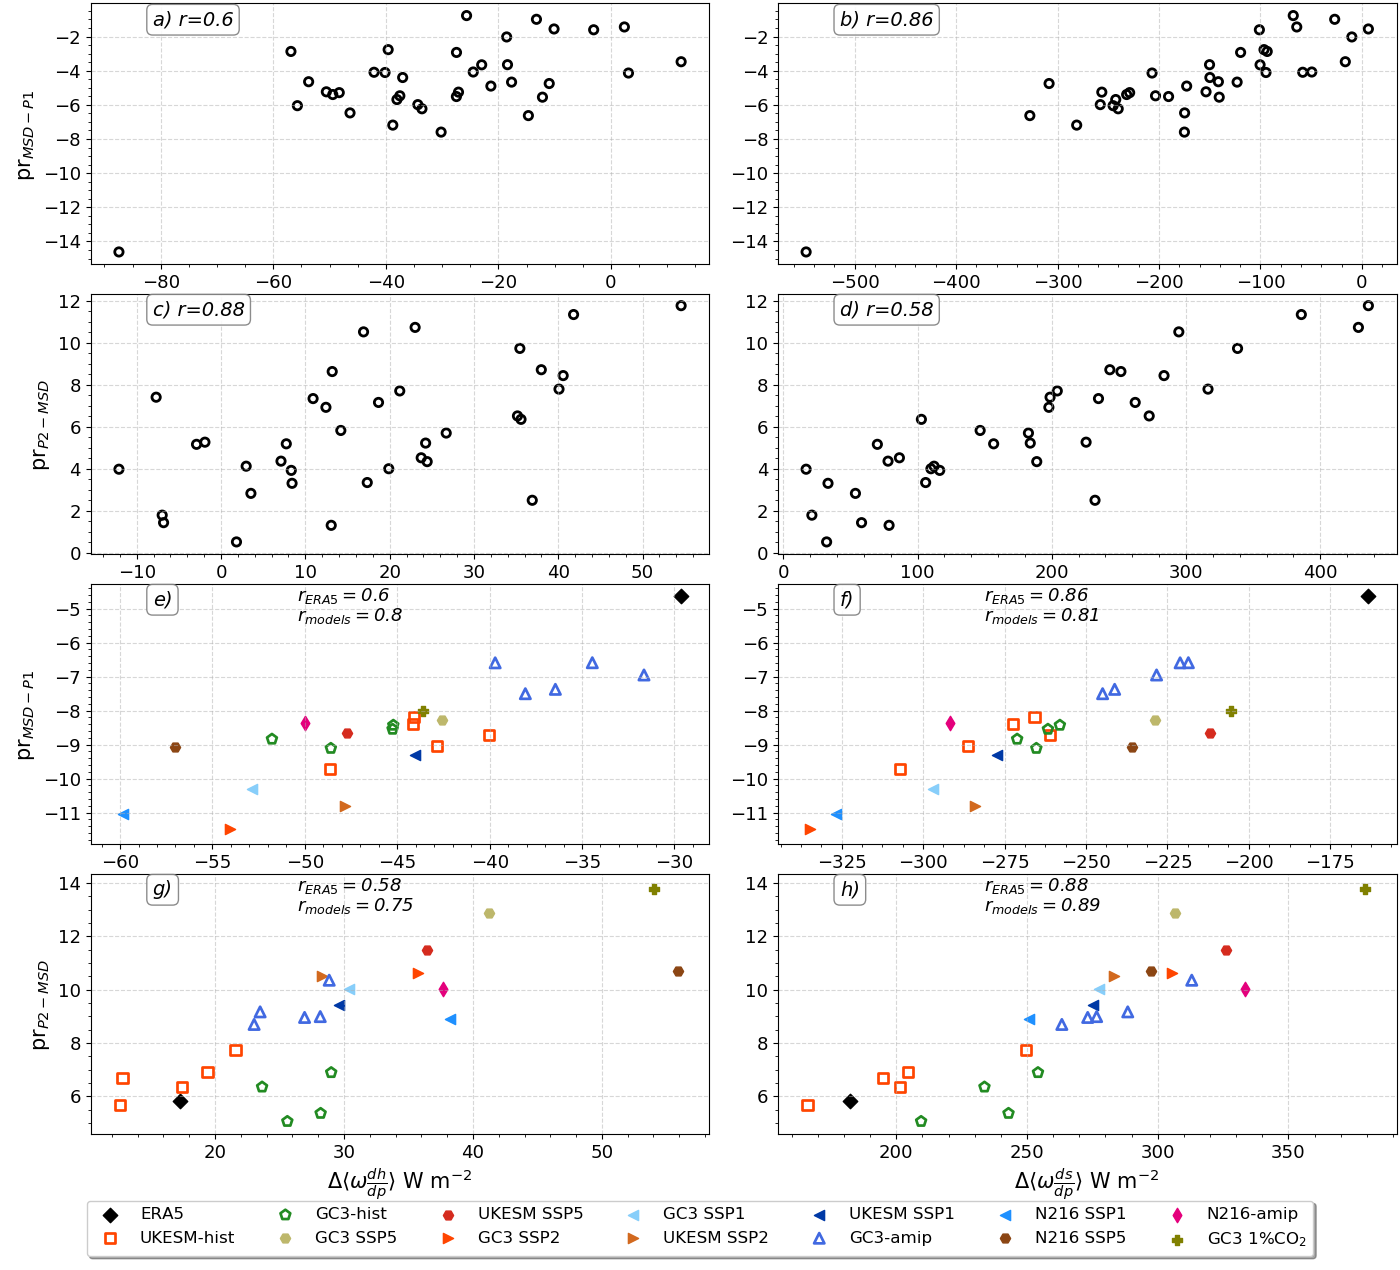
\includegraphics[width=\linewidth]{figures/thermo_scatter}
\caption[Scatterplot of the vertical advection of dry and moist static energy against precipitation]{Scatterplot of the relationship between the area-averaged mean vertical advection of dry and moist static energy and precipitation over the MSD region. In panels a, d, each dot represents the differences in the mean values between a) MSD-P1 and (d) P2-MSD for precipitation in the y-axis and vertical advection of $h$ and $s$ in the x-axis. In the rest of the panels, the differences are shown for the dataset-mean for all years in each dataset.    }
\label{fig:thermo_scatter}
\end{figure}

 The most noteworthy variations of $M_v$ associated with the MSD timings occur over the western coast of  Mexico, the Gulf of Mexico and the Caribbean. From the first peak period to the drier MSD period, $M_v$ decreases in these regions and then increases again from the dry period to the wetter second peak period. Negative and minimum $M_v$ is then found during the MSD period over most of the so-called Intra-Americas Seas region. This result is important because these changes point to seasonal variations in the relationship between convection and the large-scale dynamics \citep{raymond2009}, including the shape of the vertical velocity profile.

The horizontal advection term and the surface fluxes also show notable differences associated with the MSD timings (Figure \ref{fig:intudothanom}). In the MSD-P1 period, decreased surface fluxes in the easternmost Pacific Ocean are observed in the three simulations and, to a lesser degree, in ERA5. These differences suggest that in the models, surface fluxes decrease as precipitation decreases from the wet first peak period to the dry MSD period. In the simulations, these negative surface flux anomalies are collocated with negative differences of the horizontal advection of MSE term. 

%The horizontal advection term shows different results for ERA5 and the


\begin{figure}[t!]
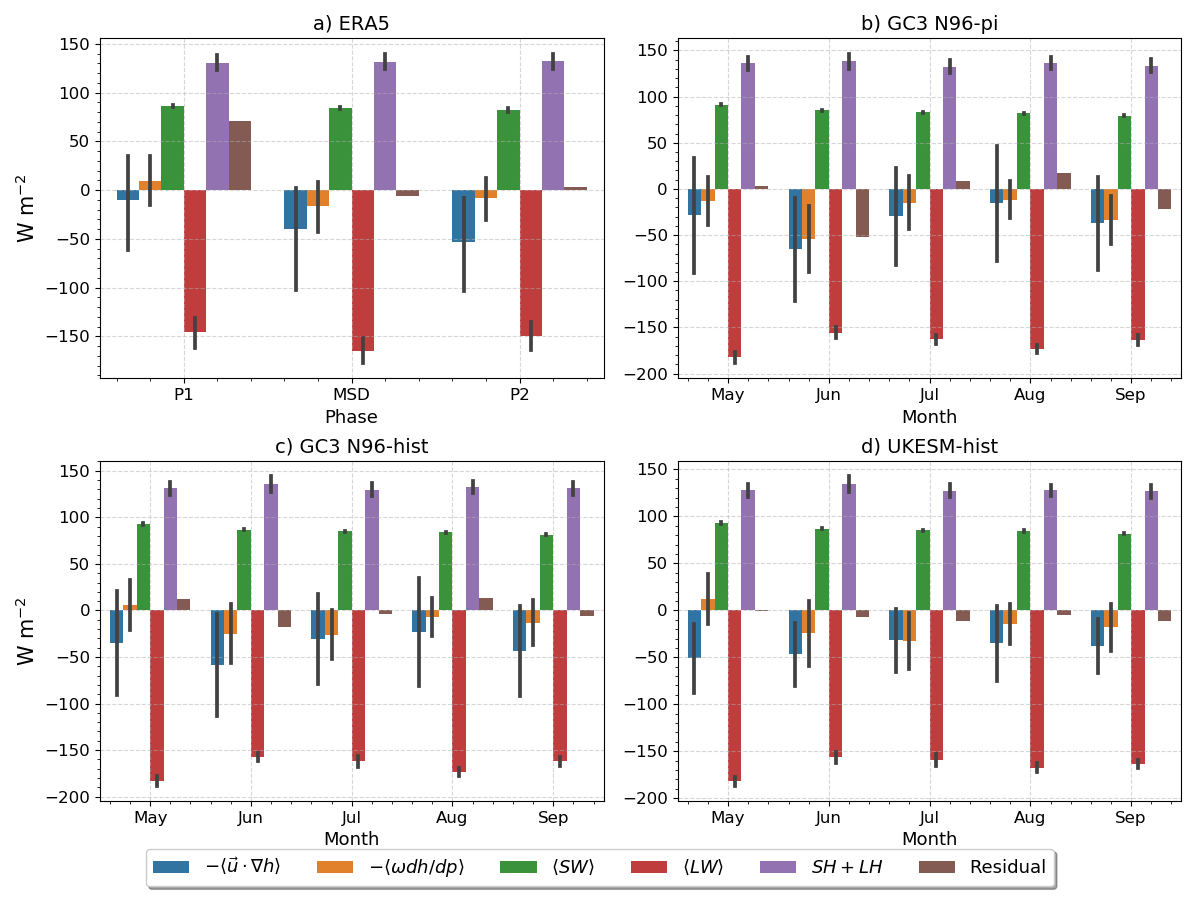
\includegraphics[width=\linewidth]{figures/mse_barplot_era5}
\caption[Barplots of MSE budget terms]{Barplots of the area and time-averaged MSE budget terms: horizontal advection ($\langle \vec{u}\cdot\nabla h \rangle$) and vertical advection ($\langle \omega dh/dp \rangle$), longwave ($\langle LW \rangle$) and shortwave($\langle SW \rangle$) and the sum of sensible ($SH$) and latent heat ($LH$) fluxes. (a) shows the budget terms computed from ERA5 in the MSD region in the P1, MSD and P2 periods. (b-d) show the monthly-mean values of the budget terms. }
\label{fig:thermo_barplot}
\end{figure}

A key question then is how the MSE budget equation is balanced in the different stages of the seasonal cycle, i.e., which terms balance the horizontal and vertical advection of MSE during the early and late wet periods and in the MSD period. 
Figure \ref{fig:thermo_barplot} shows the mean values of each budget term in the MSD in ERA5 and the simulations. The results in the simulations are shown per month because the radiative heating data from the CMIP6 archive was only available for monthly-mean frequencies.

In ERA5 (Fig. \ref{fig:thermo_barplot}a), the positive contributions of MSE from the shortwave heating and the surface fluxes are balanced mostly by the negative contribution from the longwave heating (radiative cooling of the column)  and to second order by the horizontal and vertical advection terms. 
The differences in the budget terms between the P1, MSD and P2 periods are most pronounced for the vertical and horizontal advection terms which total contribution increases during the MSD compared to the other two periods. However, from P1 to the MSD stage, the longwave radiative heating notably decreases and increases again from the MSD to P2 periods whereas the shortwave heating term appears to change very little between the stages of the rainy season.

In the CMIP6 simulations (Fig. \ref{fig:thermo_barplot}b-d), a similar balance is observed with the largest contributions arising from the terms of radiative heating and surface fluxes. 
From May to September some seasonal variations in each term are observed, for example, stronger longwave cooling in May than in June-July. The vertical advection term also increases notably during the early rainy season (June-July) compared to the rest of the wet season. As in ERA, the contribution from the vertical advection term increases during the MSD with minima found in June or July in all the simulations. 
The horizontal advection increases during the months of the two peak of precipitation (May and September) and decreases during the MSD. 


The scatter of the relationship between precipitation and the vertical advection of dry and moist static energy during the wet season (Figure \ref{fig:thermo_scatter}) indicates that the shape of the vertical profile of the vertical velocity is stronly linked to precipitation variations, both in ERA5 as in the simulations. Figure \ref{fig:thermo_scatter}a, d shows that the interannual variability of vertical advection of dry and moist static energy in ERA5 is strongly related to interannual variations in the precipitation changes during the MSD. Negative differences of $\langle \omega dh/dp \rangle$ and $\langle \omega ds/dp \rangle$ are observed in MSD-P1 panel, in agreement with the previous composite analysis whereas increases of these terms occur from the MSD period to the second peak period in ERA5 and in the experiments. Specifically, $\langle \omega ds/dp \rangle$ is the term that best explains interannual variability of the strength of the MSD, measured by the difference MSD-P1 in ERA5. 
The budget analysis shows that the variability of the horizontal advection and longwave heating terms within the rainy season is stronger than for the shortwave heating and surface fluxes. 
This evidence suggests that LW CRE and moisture transport may be more important than surface fluxes of total shortwave incoming to the troposphere, which supports the mechanism that links the CLLJ to the precipitation in the MSD. These budget terms could also be interpreted as evidence that cloud-radiative feedback mechanism and the solar declination angle are less likely to explain the MSD.

\section{Summary and discussion}\label{sq:sumdiscuss}

The Midsummer drought (MSD) is a key element of past, present and future climates of southern Mexico, northern Central America and the Caribbean with important implications for agriculture and water management \citep{hellin2017,de2018,harvey2018}. However, a complete description of the physical mechanisms that explain the spatial and temporal variability of the MSD is not yet clear. This lack of understanding is magnified when investigating the MSD in global climate models that are used for projections of future climate, as little is known as to why only some models can reproduce the MSD \citep{ryu2014}.


This chapter tackled these shortcomings in the literature by investigating the processes that are linked to the MSD in CMIP6 experiments of the MOHC models, an investigation that was motivated by the two previous chapters which showed that these models reasonably reproduced the main features of the MSD signal.
The first contribution of this chapter is the diagnosis of MSD timings and patterns on a sub-monthly scale, a step forward from previous studies that diagnosed the MSD on monthly-mean timescales, possibly missing key information in the process. 
For this purpose, the wavelet transform method (WT; Chapter \ref{ch:5-wvt}) was used to determine the timings of the MSD on a 5-day (pentad) scale. 


The WT method proved useful to separate the wet season in each dataset into three stages: the first and second peak periods (P1 and P2) and the drier period (MSD). 
This approach using the WT method was able to reproduce the so-called MSD pattern reported in previous studies \citep{zermeno2019,zhao2020} using various diagnostics such as OLR, $\omega$ and the low-level wind flow. This pattern is characterised by strong changes to the zonal wind flow crossing from the Caribbean Sea into the easternmost Pacific Ocean, as well as by anomalous vertical velocities found west of the coast at around 125$^\circ$W, in agreement with previous findings \citep{herrera2015,zermeno2019}. 

% These composites show that the MSD pattern is not a local feature in a small region but covers a wider region from central Mexico south to Belize, Guatemala, El Salvador, Honduras, Nicaragua, and northern Costa Rica including regions over the ocean in the easternmost Pacific Ocean, the Gulf of Mexico and the western Caribbean Sea, which ag.  
The chapter first evaluates key climate features in the region such as the seasonal cycle of the Caribbean Low-Level Jet (CLLJ) and East Pacific SSTs. Results show that the simulations agree well with the observed seasonal cycle and that the experiments show very similar MSD patterns to observations. 
The following sections in the chapter test three of the leading hypotheses put forth to explain the MSD, this investigation is the second key contribution from this chapter.
 Each hypothesis is evaluated using the WT method in two different ways. The first question was whether a hypothesis could explain  the interannual variability in the strength and timing of the MSD  in ERA5. The second approach focused on the CMIP6 experiments and aimed to test whether the elements of each hypothesis could explain the differences in precipitation at each stage of the seasonal cycle between the realizations.
 
 The first mechanism proposed by \cite{magana1999} argues that SST-cloud-radiative feedbacks explain the MSD. In this hypothesis, the SSTs in the East Pacific should also exhibit a bimodal seasonal cycle, with a second peak in SSTs found in September. Even though \cite{magana2005} analysed this for a specific year and found no evidence of a second peak in SSTs, no study to date robustly evaluated whether observations or models confirm their hypothesis. This chapter provides evidence that in ERA5, SSTs not only do not increase at the later stages of the summer but rather decrease. While the seasonal cycle in the simulations do show a two peak structure, the composite analysis shows that as precipitation transitions from the drier MSD to the second peak periods, SSTs decrease in the Pacific coast of Central America, in contrast to the prediction of the SST-cloud feedback mechanism. No evidence is found that the variability of the East Pacific SSTs is directly associated with the precipitation over the MSD region in ERA5 or in the CMIP6 experiments. 

 
The feedback mechanism also suggests that the second peak is a result of a second increase in downwelling shortwave radiation at the surface that results from cloud cover during the drier MSD.
The solar declination angle mechanism of \cite{karnauskas2013} also suggests that shortwave absorption has two peaks in the seasonal cycle, which leads to the two precipitation peaks. The shortwave absorption at the surface does show a bimodal seasonal cycle in ERA5 and in the simulations, as predicted by these two mechanisms.

 However, the interannual variability in ERA5 and inter-experiment differences in the absorbed shortwave at the different stages of the seasonal cycle cannot explain the changes over precipitation. Moreover, no significantly positive correlation is found between the shortwave absorption at the surface and precipitation at any lags but rather a strong anticorrelation signal is found, which is a result of stronger convective activity leading to more cloud cover and less downwelling shortwave at the surface. 
 Therefore, while this chapter found some evidence of strong correlations between SW and precipitation, there is little evidence found that the SW drives precipitation, as argued by the solar declination angle mechanism.

Cloud-radiative effects (CRE) are known to be key for precipitation in monsoon regions and the central argument of \cite{magana1999} is that precipitation and CRE (at the surface) are part of a feedback mechanism that explains the MSD. This chapter presents the first regional evaluation of the net CRE at the surface as well as the long-wave and short-wave contributions. The net CRE at the surface over the wet season is negative following the regions of maximum precipitation, i.e., the East Pacific ITCZ and the MSD region reaching values of -100 W m$^{-2}$ over the core ITCZ region in both the models and ERA5.

 The net CRE is dominated by the short-wave component that acts to cool the surface due to the effect of cloud cover associated with convection. Over the MSD region, the net, short-wave and long-wave CRE at the surface show a bimodal regime that closely follows the evolution of precipitation. Finally, an experiment part of CFMIP in which the long-wave effects of clouds are turned-off from the radiative scheme shows that the longwave radiative effects are key for monsoon precipitation in Central America and southern Mexico,  where long-wave effects are decoupled from the simulation, shows that the long-wave component of CRE are key for sustaining the monsoon circulation and precipitation irrespective of the bimodal MSD signal.

This section showed that CRE have a strong seasonal cycle associated with the MSD in ERA5 and the MOHC experiments. However, further research into CRE in present and future climates in the region is warranted, for example, further work could include a detailed examination of the CRE at the top of atmosphere and at the surface in the MSD, particularly to understand the relationship between CRE and the large-scale circulation, and how this relationship is different over land in Mesoamerica than over the Caribbean Sea and the East Pacific Ocean.

One alternative hypothesis is that the MSD is caused by the modulation of the transport of moisture by the CLLJ \citep{herrera2015,zermeno2019,martinez2019}. The integrated moisture flux convergence and the total column water content are found to better explain observed and simulated differences in precipitation, compared to the previous hypotheses. Evidence is presented that the low-level wind flow variations on the west coast of Central America is linked to the variations in the strength and direction of the CLLJ. 
Changes to the CLLJ and moisture convergence allow skillful predictions of precipitation changes at the end of the MSD period but these are less skilful for changes at the start of the MSD. 

A moist static energy (MSE) budget is implemented to investigate whether this technique could provide additional insight into the mechanisms of the MSD. The total column MSE, as well as the vertical advection terms of the budget show a clear bimodal signal that closely follows that of precipitation. The vertical advection of dry and moist static energy are found to have the strongest relationship to the interannual variability and the inter-experiment differences of precipitation in the MSD region. 

In particular, $\langle \omega ds/dp \rangle$ is able to explain interannual variability in ERA5 as well as the precipitation differences between the range of experiments considered in this chapter. While these results do not directly point to any theory or hypothesis, the strong correlations in reanalysis and simulations indicate that MSE budgets would be useful in future research to better understand the key mechanism underpinning the MSD. Specifically, this result points to a possible modulation of the strength of convection by the shape of the vertical velocity profile, which is the key modulator of these terms. How the vertical velocity profile changes during the rainy season, and whether there are notable trends in ERA5 or significant changes between historical and Scenario experiments warrants further research.
 
 
